%

\PassOptionsToPackage{table,xcdraw}{xcolor}

\documentclass[10pt,twocolumn,letterpaper]{article}

%%%%%%%%% PAPER TYPE  - PLEASE UPDATE FOR FINAL VERSION
\usepackage{cvpr}              % To produce the CAMERA-READY version
%

\usepackage{booktabs}
\usepackage{graphicx}
\usepackage{multirow}
\usepackage{makecell}
%\usepackage[table,xcdraw]{xcolor}
\usepackage{amssymb}
\usepackage{amsmath}
\usepackage[linesnumbered,ruled,vlined]{algorithm2e}
\usepackage{pifont}

\usepackage{listings}

\lstset{
    backgroundcolor=\color{codebackgroundcolor},%代码块背景色为浅灰色\color{customcolor}
    rulesepcolor= \color{gray}, %代码块边框颜色
    breaklines=true,  %代码过长则换行
    numbers=left, %行号在左侧显示
    numberstyle= \small,%行号字体
    %keywordstyle= \color{blue},%关键字颜色
    commentstyle=\color{gray}, %注释颜色
    frame=shadowbox%用方框框住代码块
}


% Import additional packages in the preamble file, before hyperref
%
% --- inline annotations
%
\newcommand{\red}[1]{{\color{red}#1}}
\newcommand{\todo}[1]{{\color{red}#1}}
\newcommand{\TODO}[1]{\textbf{\color{red}[TODO: #1]}}
% --- disable by uncommenting  
% \renewcommand{\TODO}[1]{}
% \renewcommand{\todo}[1]{#1}



%
\definecolor{cvprblue}{rgb}{0.21,0.49,0.74}
\usepackage[pagebackref,breaklinks,colorlinks,allcolors=cvprblue]{hyperref}

%%%%%%%%% PAPER ID  - PLEASE UPDATE
\def\paperID{1770} % *** Enter the Paper ID here
\def\confName{CVPR}
\def\confYear{2025}

%%%%%%%%% TITLE - PLEASE UPDATE
\title{Omnidirectional Multi-Object Tracking}

%%%%%%%%% AUTHORS - PLEASE UPDATE
\author{
Kai Luo$^{1,}$\thanks{Equal contribution} \quad Hao Shi$^{2,*}$ \quad Sheng Wu$^{1}$ \quad Fei Teng$^{1}$ \quad Mengfei Duan$^{1}$ \quad Chang Huang$^{1}$\\Yuhang Wang$^{1}$ \quad Kaiwei Wang$^{2}$ \quad Kailun Yang$^{1,}$\thanks{Correspondence: kailun.yang@hnu.edu.cn}\\
$^{1}$Hunan University \quad $^{2}$Zhejiang University\\
}

% teaser
\let\oldtwocolumn\twocolumn
\renewcommand\twocolumn[1][]{%
    \oldtwocolumn[{#1}{
    \begin{center}
    \vskip-6ex
        \centering
        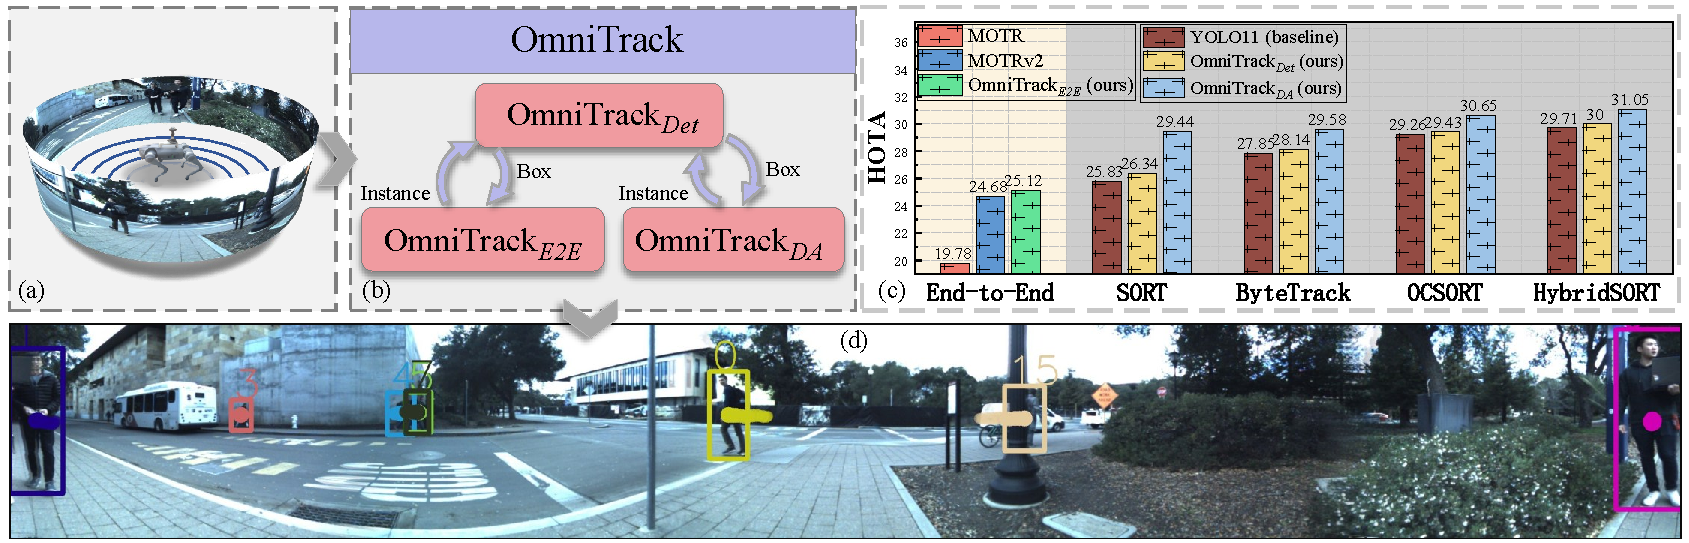
\includegraphics[width=1.0\textwidth]{imgs/fig_1v10.pdf}
        \vskip-2ex
        \captionof{figure} {{Comparison of OmniTrack's overall structure and performance. (a) shows the input panoramic image. (b) illustrates the proposed OmniTrack method. (c) presents a performance comparison with other multi-object tracking algorithms. (d) visualizes tracking results. 
        }}
        \label{fig:1}
    \end{center}
    }]
}

\begin{document}
\maketitle

\begin{abstract}
Fine-tuning provides an effective means to specialize pre-trained models for various downstream tasks. However, fine-tuning often incurs high memory overhead, especially for large transformer-based models, such as LLMs. While existing methods may reduce certain parts of the memory required for fine-tuning, they still require caching all intermediate activations computed in the forward pass to update weights during the backward pass. In~this work, we develop \method, a method to reduce memory usage,  specifically the memory to store intermediate activations, in the fine-tuning of transformer-based models. During the backward pass, \method approximates the gradient computation by backpropagating through just a subset of input tokens. Thus, with \method, only a subset of intermediate activations are cached during the forward pass. Also, \method can be easily combined with existing methods like LoRA, further reducing the memory cost. We evaluate our approach on pre-trained transformer models with up to billions of parameters, considering the performance on multiple downstream tasks such as text classification and question answering in a few-shot learning setup. Overall, \method achieves performance on par with full fine-tuning or representative memory-efficient fine-tuning methods,  while greatly reducing the memory footprint, especially when combined with other methods with complementary memory reduction mechanisms. We hope that our approach will facilitate the fine-tuning of large transformers,  in specializing them for specific domains or co-training them with other neural components from a larger system. Our code is available at \githubURL.
\blfootnote{\textbf{*} Equal contribution}
\end{abstract}
    
\section{Introduction}
\label{sec:intro}

\begin{figure*}[t!]
    \centering
    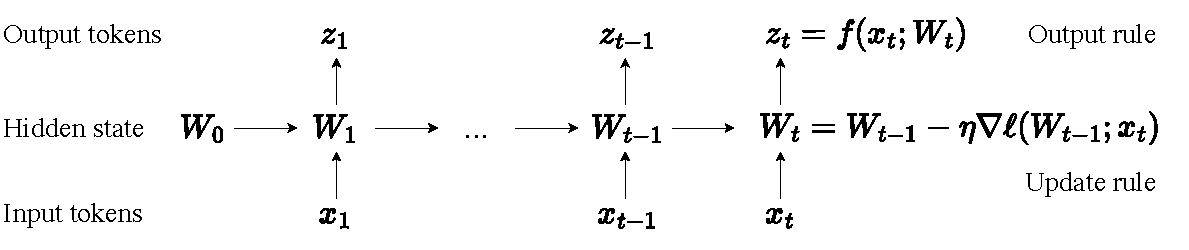
\includegraphics[width=0.8\textwidth]{figs/simple_teaser.pdf}
    \caption{All RNN layers can be expressed as a hidden state that transitions according to an update rule.
    The key idea in \cite{sun2024ttt} is to make the hidden state itself a model $f$ with weights $W$, and the update rule a gradient step on the self-supervised loss $\ell$.
    Therefore, updating the hidden state on a test sequence is equivalent to training the model $f$ at test time. 
    This process, known as Test-Time Training (TTT), is programmed into TTT layers. 
    Figure and caption taken from \cite{sun2024ttt}.
    }
    \label{fig:ttt-layer}
\end{figure*}

Despite the remarkable progress in visual and physical realism, state-of-the-art video Transformers are still generating mostly short clips of single scenes without complex stories.
At the time of writing (March 2025), the maximum length of public APIs for video generation is 20 seconds for Sora (OpenAI), 16 seconds for MovieGen (Meta), 10 for Ray~2 (Luma), and 8 for Veo~2 (Google).
None of these APIs can autonomously generate complex multi-scene stories.

A fundamental challenge behind these technical limitations is long context, because the cost of self-attention layers in Transformers increases quadratically with context length.
This challenge is especially acute for video generation with dynamic motion, whose context cannot be easily compressed by a tokenizer.
Using a standard tokenizer, each of our one-minute videos requires over 300k tokens in context. 
With self-attention, generating a one-minute video would have taken $11\times$ longer than generating 20 videos of 3 seconds each, and training would have taken $12\times$ longer.

To address this challenge, recent work on video generation has investigated RNN layers as an efficient alternative to self-attention, because their cost increases linearly with context length~\cite{wang2024lingenhighresolutionminutelengthtexttovideo}.
Modern RNN layers, especially variants of linear attention~\cite{schmidhuberlinearattn, katharopoulos2020lineartransformers} such as Mamba~\cite{gu2024mamba, dao2024mamba2} and DeltaNet~\cite{schlag2021deltanet, yang2025gateddeltanetworksimproving}, have shown impressive results for natural language tasks.
However, we have yet to see long videos with complex stories or dynamic motion generated by RNNs.
Videos (\href{https://lineargen.github.io/}{link}) in \cite{wang2024lingenhighresolutionminutelengthtexttovideo} are high resolution and one-minute long, but contain only single scenes and slow motion, let alone complex stories.

We believe that these RNN layers generate less complex videos because their hidden states are less expressive.
RNN layers can only store past tokens into a hidden state of fixed size, which is only a matrix for linear attention variants such as Mamba and DeltaNet.
It is inherently challenging to compress hundreds of thousands of vectors into a matrix with only thousands in rank.
As a consequence, these RNN layers struggle to remember the deep relationships between distant tokens.

We experiment with an alternative class of RNN layers whose hidden states themselves can be neural networks. Specifically, we use two-layer MLPs with 2$\times$ more hidden cells and richer nonlinearities than the linear (matrix) hidden states in linear attention variants.
Since the neural network hidden states are updated by training even on test sequences, these new layers are called Test-Time Training (TTT) layers~\cite{sun2024ttt}.

We start from a pre-trained Diffusion Transformer (CogVideo-X 5B \cite{hong2023cogvideo}) that could only generate 3-second short clips at 16 fps (or 6 seconds at 8 fps).
Then, we add TTT layers initialized from scratch and fine-tune this model to generate one-minute videos from text storyboards. 
We limit the self-attention layers to 3-second segments so their cost stays manageable.
With only preliminary systems optimization, our training run takes the equivalent of 50 hours on 256 H100s.

We curate a text-to-video dataset based on $\approx$ 7 hours of \textit{Tom and Jerry} cartoons with human-annotated storyboards.
We intentionally limit our scope to this specific domain for fast research iteration.
As a proof-of-concept, our dataset emphasizes complex, multi-scene, and long-range stories with dynamic motion, where progress is still needed; it has less emphasis on visual and physical realism, where remarkable progress has already been made.
We believe that improvements in long-context capabilities for this specific domain will transfer to general-purpose video generation.

Compared to strong baselines such as Mamba 2~\cite{dao2024mamba2}, Gated DeltaNet~\cite{yang2025gateddeltanetworksimproving}, and sliding-window attention layers, TTT layers generate much more coherent videos that tell complex stories with dynamic motion, leading by 34 Elo points in a human evaluation of 100 videos per method.
For context, GPT-4o scores 29 Elo points over GPT-4 Turbo in LMSys Chatbot Arena~\cite{chiang2024chatbot}.

Sample videos, code and annotations are available at:
\url{https://test-time-training.github.io/video-dit}
\section{Related Work}
\label{sec:related_works}


\noindent\textbf{Panoramic scene understanding.}
Panoramic perception enables a holistic understanding of a 360{\textdegree} scene in a single shot~\cite{gao2022review,chen2024360+,dong2024panocontext,ehsanpour2022jrdb_act,jiang2024minimalist,jiang2022annular,ai2022deep}. 
Main areas include 
panoramic scene segmentation~\cite{teng2024360bev,zheng2024360sfuda++,cao2024occlusion,zheng2024semantics,yan2023panovos,jaus2021panoramic_panoptic,jaus2023panoramic_insights}, 
panoramic estimation~\cite{bai2024glpanodepth,ai2024elite360d,wang2022bifuse++,shen2022panoformer,chang2023depth_neural}, 
panoramic layout estimation~\cite{yu2023panelnet,shen2023disentangling,ling2023panoswin}, 
panoramic generation~\cite{zhou2025dreamscene360,wang2024360dvd,li2023panogen}, 
and panoramic flow estimation~\cite{shi2023panoflow,li2022deep}, \etc~\cite{park2024fully,kim2024fully,fan2024learned,han2022panoramic_activity}.
Researchers typically unfold panoramas into equirectangular projections or polyhedral projections to adapt algorithms designed for limited-FoV data~\cite{jiang2021unifuse,wang2022bifuse++,li2022deep}. 
They also apply techniques such as deformable convolutions to handle severe distortions in high-latitude regions~\cite{shi2023panoflow,zhang2024behind}.

Recently, researchers have recognized the advantages of omnidirectional images for tracking, particularly their ability to maintain continuous observation of targets without the out-of-view issues present in limited field-of-view setups.
Jiang~\etal~\cite{jiang2021500} propose a $500$FPS omnidirectional tracking system using a three-axis active vision mechanism to capture fast-moving objects in complex environments.
The 360VOT benchmark~\cite{huang2023360vot} is introduced for omnidirectional object tracking, focusing on spherical distortions and object localization challenges.
Huang~\etal~\cite{huang2024360loc} present 360Loc for omnidirectional localization that tackles cross-device challenges by generating lower-FoV query frames from 360{\textdegree} data. 
Another work by Xu~\etal~\cite{xu2024360vots} introduces an extended bounding FoV (eBFoV) representation to alleviate spherical distortions in panoramic videos.
Unlike previous methods, this work first explores extremely challenging panoramic-FoV and intense-motion panoramic tracking for mobile robots, \eg, aiming to enhance the robot’s spatiotemporal understanding of objects in its surroundings.

\noindent\textbf{Multi-object tracking.}
Object tracking primarily follows two paradigms: Tracking-By-Detection (TBD)~\cite{Chen_2024_CVPR,Du_2024_CVPR,qin2024towards,nettrack2024cvpr,huang2024deconfusetrack,lv2024diffmot,li2023ovtrack,qin2023motiontrack} and End-To-End (E2E)~\cite{ding2024adatrack,li2023end,MeMOTR,zeng2022motr}. 
Among these, TBD is currently one of the most prevalent, with frameworks following the design principles of SORT~\cite{wojke2017simple}. 
First, the detection network~\cite{yolox2021,carion2020end} is used to locate bounding boxes for objects, then the target's current position is predicted based on its historical trajectory, and the predicted results are associated with detection results~\cite{kuhn1955hungarian}. 
Many subsequent works have refined this approach: DeepSORT~\cite{li2022deep} introduced a ReID model to incorporate appearance information for association, and ByteTrack~\cite{zhang2022bytetrack} designed a confidence-based, stage-wise association strategy. 
Other methods~\cite{aharon2022bot,yi2024ucmc,du2023strongsort} introduced motion compensation modules to mitigate camera motion, and OC-SORT~\cite{cao2023observation} optimized the motion estimation module. Additionally, E2E methods have continued to evolve. 
TrackFormer~\cite{meinhardt2021trackformer} and MOTR~\cite{zeng2022motr} proposed transformer-based, End-to-End tracking approaches. 
Recent improvements~\cite{zhang2023motrv2, lv2024diffmot} have enhanced detector performance and improved data association accuracy in occlusion scenarios. 
Unlike existing methods that focus on narrow-FoV pinhole camera data with linear sensor motion, we address the challenges of MOT in panoramic-FoV scenarios, tackling issues such as geometric distortion and complex motion.
\begin{figure}[!t]
  \centering
  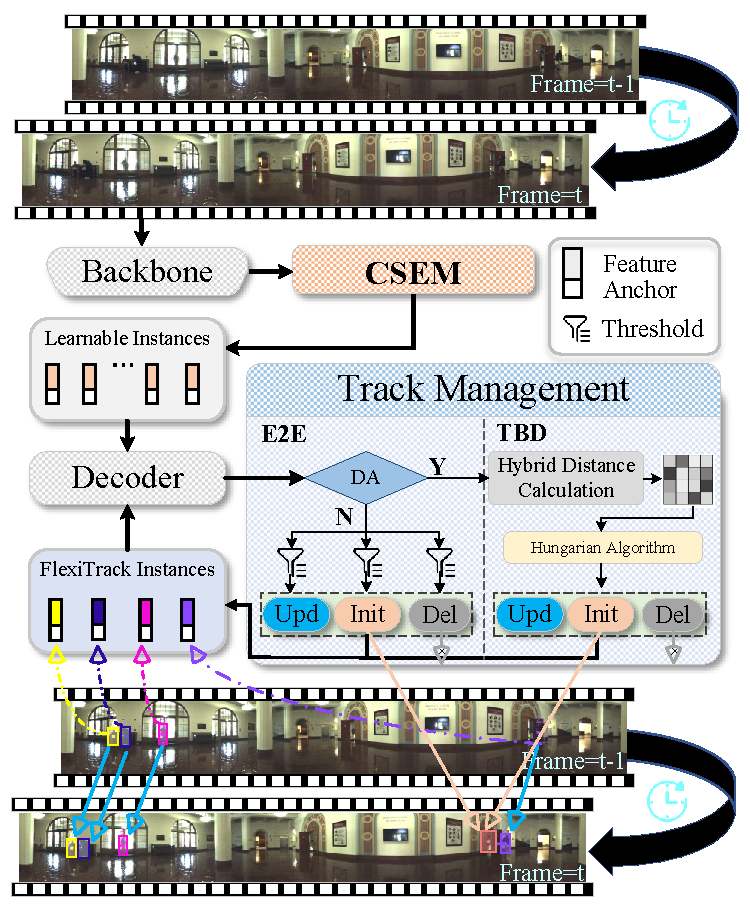
\includegraphics[width=0.48\textwidth]{imgs/id_assignment_single_v2.pdf}
  \vskip -1ex
  \caption{The proposed OmniTrack pipeline. \textbf{CSEM} refers to the CircularStatE Module \ref{subsec:CSEM}
, \textbf{DA} stands for data association, \textbf{E2E} denotes the End-to-End tracking paradigm, \textbf{TBD} refers to the Track-By-Detection tracking paradigm, \textbf{Upd} refers to updating tracks, \textbf{Init} to initializing tracks, and \textbf{Del} to deleting tracks.}

  \label{fig:pipeline}
  \vskip -2ex
\end{figure}

\begin{algorithm}
\caption{OmniTrack Inference Process}
\algorithmfootnote{In \textcolor{codegreen}{green} is the key of our method. }

\label{alg:Omnitrack}
\footnotesize
\KwIn{
A Panoramic video/image sequence $\texttt{V}$
%
}

\KwOut{
Tracks $\mathcal{T}$ of the video/image sequence
%
}

Initialization: $\mathcal{T} \leftarrow \emptyset$\;

Define the Initialize threshold $\mathcal{\tau}_\mathcal{I}$ \;
Define the Update threshold  $\mathcal{\tau}_\mathcal{U}$ \;


\For{frame $f_k$ in $\texttt{V}$}{
\tcc{As shown in Fig. \ref{fig:pipeline}}

$\{\mathcal{S}_3, \mathcal{S}_4, \mathcal{S}_5\} \leftarrow \texttt{Backbone}(f_k)$ \;

\textcolor{codegreen}{$ \mathcal{I}_L \leftarrow  \texttt{CSEM}(\{\mathcal{S}_3, \mathcal{S}_4, \mathcal{S}_5\})$} \;

\textcolor{codegreen}{$ \mathcal{I}_F \leftarrow  \mathcal{T}_{f_{k-1}}$} \;

$ \textcolor{codegreen}{\mathcal{D}_k^F}, \mathcal{D}_k^L \leftarrow  \texttt{Decoder} ( \textcolor{codegreen}{\mathcal{I}_F}, \mathcal{I}_L) $ \;

\BlankLine
\BlankLine
    \If{$\texttt{DA}$}{
        \tcc{Data Association}
	
        $\mathcal{C} \leftarrow  \texttt{Distance Calculation}(\textcolor{codegreen}{{\mathcal{D}_k^F}}+ \mathcal{D}_k^L, \mathcal{T}_{f_{k-1}})$ \;

        $\{\texttt{Update, Initialize, Delate} \} \leftarrow \texttt{Hungarian Algorithm}(\mathcal{C})$ \;
    
        $\mathcal{T}_{f_{k}} \leftarrow \{\texttt{Update, Initialize, Delete} \} $
    }
    
    \Else{
        \tcc{End-to-End}
        
            \textcolor{codegreen}{\For{$d$ in $ \{\mathcal{D}_k^F \cup \mathcal{D}_k^L$\} }{
	            \If{$ d \in \mathcal{D}_k^F \And d.score > \mathcal{\tau}_\mathcal{U} $}{
	               $\texttt{Update} \leftarrow  d$ \;
                }
                    \If{$ d \in \mathcal{D}_k^L \And d.score > \mathcal{\tau}_\mathcal{I}  $}{
	               $\texttt{Initialize } \leftarrow  d$ \;
                }
                \Else{
                    $\texttt{Delete} \leftarrow  d$ \;
                }
            }
        }
        $\mathcal{T}_{f_{k}} \leftarrow \{\texttt{Update, Initialize, Delete} \} $
    }
}


\textbf{Return}: $\mathcal{T}$

%

%
\end{algorithm}

\section{OmniTrack: Proposed Framework}
%

In this section, we introduce OmniTrack, a panoramic multi-object tracking framework that addresses the unique challenges in panoramic-FoV images, including extensive search spaces, geometric distortion, resolution loss, and lighting inconsistencies. 
OmniTrack is designed with a feedback mechanism to iteratively refine object detection, integrating trajectory information back into the detector to enhance tracking stability across panoramic-FoV scenes (Sec.~\ref{subsec:Framework}).
%
Specifically, we propose the OmniTrack framework, which consists of three key components:

%
\begin{itemize}
    \item \textbf{Tracklets Management} (Sec.~\ref{subsec:Tracklets Management}): Manages object trajectory lifecycles and provides temporal priors to the perception module.
    \item \textbf{FlexiTrack Instance} (Sec.~\ref{subsec:Temporal Query}): Rapidly locates and associates objects across the panoramic view by leveraging temporal context.
    \item \textbf{CircularStatE Module} (Sec.~\ref{subsec:CSEM}): Mitigates geometric distortion and improves consistency across the panoramic FoV, enhancing feature reliability.
\end{itemize}

%
\subsection{Feedback Mechanism}
\label{subsec:Framework}
%

The OmniTrack framework, illustrated in Fig.~\ref{fig:pipeline}, incorporates a feedback mechanism that iteratively refines detections by integrating trajectory information back into the detector. This mechanism operates on the principle of reducing information entropy, thereby enhancing stability in Panoramic-FoV and improving MOT performance.

%

In traditional MOT~\cite{zhang2022bytetrack,cao2023observation,du2023strongsort,aharon2022bot}, detection and association are decoupled, leading to higher entropy as each frame’s detection \( H(x_t) \) is calculated independently:
\begin{align}
H(x_t) = -\sum_{i=1}^{n} P(x_t^i) \log P(x_t^i),
\end{align}
where \( x_t^i \) denotes the position of the \( i \)-th target in frame \( t \), with probability distribution \( P(x_t^i) \). The global association entropy~\(H(\{y_t\}) \) depends on the joint probability distribution of target positions across all frames:
\begin{align}
H(\{y_t\}) = -\sum_{i=1}^{n} &P(\{x_1^i, x_2^i, \dots, x_T^i\}) \notag  \\ \times  & \log P(\{x_1^i, x_2^i, \dots, x_T^i\}). 
\label{eq:2}
\end{align} 
The cumulative entropy across all frames, accounting for independent matching, is formulated as:
\begin{align}
H_{\text{independent}} = \sum_{t=1}^{T} H(x_t) + H(\{y_t\}).
\end{align}
%
In contrast, OmniTrack’s feedback mechanism allows detections from frame \( t{-}1 \) to inform those in frame \( t \), reducing per-frame uncertainty. Specifically, the conditional entropy of frame \( t \), given prior feedback \( y_{t-1} \), is:
\begin{align}
H(x_t | y_{t-1}) = -\sum_{i=1}^{n} P(x_t^i | y_{t-1}^i) \log P(x_t^i | y_{t-1}^i).
\end{align}
The total entropy with feedback becomes:
\begin{align}
H_{\text{feedback}} = \sum_{t=1}^{T} H(x_t | y_{t-1}),
\end{align}
where \( H_{\text{feedback}} {<} H_{\text{independent}} \), indicating a reduction in uncertainty over time. This feedback-driven approach thus enhances tracking stability in panoramic-FoV scenarios. 

%

\label{subsec:Mamba encoder}
\begin{figure}[!t]
  \centering
  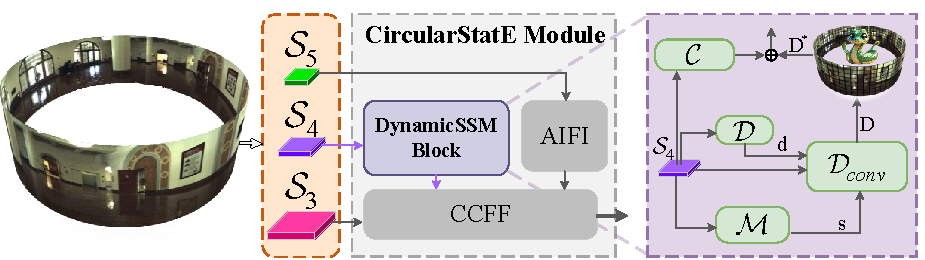
\includegraphics[width=0.48\textwidth]{imgs/CircularStatE_ModuleV4.pdf}
  \caption{The proposed \textbf{CircularStatE Module} fuses multi-scale features to generate learnable instances. The \textbf{DynamicSSM Block} mitigates distortions in panoramic-FoV images, enhancing feature stability across uneven lighting and color distributions.}
  \label{fig: CircularStatE Module}
  \vskip -2ex
\end{figure} 

\subsection{Tracklets Management}
\label{subsec:Tracklets Management}

%

To reduce uncertainty in target localization and association while incorporating temporal information, OmniTrack incorporates a Tracklets Management module. 
During training, this module caches temporal data for instances with confidence scores exceeding a threshold \(\tau\), providing historical context to improve detection consistency in subsequent frames.
During inference, Tracklets Management oversees trajectory lifecycle management by updating, deleting, or initializing instances based on their confidence scores. In scenarios without data association, trajectories are managed directly, forming OmniTrack\(_{E2E}\) (Alg.~\ref{alg:Omnitrack}, Lines 14-21). When data association is enabled, Tracklets Management utilizes TBD-based methods~\cite{cao2023observation,yang2024hybrid} to enhance tracking, referred to as OmniTrack\(_{DA}\) (Alg.~\ref{alg:Omnitrack}, Lines 10-12)

%

\subsection{FlexiTrack Instance}
\label{subsec:Temporal Query}
As described in Eq.~(\ref{eq:2}), the global association entropy is significantly high under panoramic-FoV conditions, making the association task challenging. 
%
Benefiting from the Feedback Mechanism~(Sec.~\ref{subsec:Framework}), which integrates trajectory information into the detector to reduce information entropy.
%
This approach eliminates the need for global search across the entire field of view, making it especially effective for panoramic-scale perception tasks.
Based on this insight, we introduce \emph{FlexiTrack Instance}.

%

Each FlexiTrack Instance (see Fig.~\ref{fig:pipeline}) shares the Decoder network structure with Learnable Instances, consisting of a feature vector \( \mathcal{X} {\in} \mathbb{R}^{128} \) and an anchor \( \mathcal{Y} {\in} \mathbb{R}^{128} \), as shown in Fig.~\ref{fig:pipeline}. 
By sharing the decoder, FlexiTrack Instances can seamlessly adapt to various MOT paradigms, enhancing flexibility and allowing integration across different approaches without additional modifications.
%
To enhance robustness, noise is added to both feature vectors and anchors during training, minimizing dependency on historical data and improving generalization:
\begin{align}
\mathcal{X}' = \mathcal{X} + \mathcal{N}_X, \quad \mathcal{Y}' = \mathcal{Y} + \mathcal{N}_Y, 
\end{align}
where \( \mathcal{N}_X \) and \( \mathcal{N}_Y \) represent the noise components added to the feature vector and anchor, respectively.
To initialize all FlexiTrack Instances, let \( \mathcal{I_F} \) denote the set of initial \emph{instances}, and \( N \) the total number of trajectories. 
Each instance \( \mathcal{I_F}^i \) is composed of a feature vector \( \mathcal{X}_i \) and an anchor \( \mathcal{Y}_i \), as:
\begin{align}
\mathcal{I_F} = \left\{  \mathcal{I_F} ^i \mid \mathcal{I_F}^i = (\mathcal{X}'_i, \mathcal{Y}'_i), i \in \{1, 2, \dots, N\} \right\}.
\end{align}
%
\( \mathcal{X}'_i {\in} \mathbb{R}^{d_{\mathcal{X}}} \) and \( \mathcal{Y}'_i {\in} \mathbb{R}^{d_{\mathcal{Y}}} \) are the feature vector and anchor of the \( i \)-th trajectory, 
%
with \( d_{\mathcal{X}} {=} d_{\mathcal{Y}} {=} 128 \) representing their respective dimensions.
This enables $\mathcal{I_F}$ to inherit trajectory information, guiding the perception module to quickly locate the object and establish temporal associations.

%


% 

\begin{table*}
	\centering
	\small
	\resizebox{0.98\textwidth}{!}{
		\setlength\tabcolsep{8pt}
		\renewcommand\arraystretch{1.0}
    \begin{tabular}{l|cc|cc|cccc}
        % \toprule
        % \hline
        \topline
        \rowcolor{mygray}
          & \multicolumn{2}{c|}{\textbf{Data}} & \multicolumn{2}{c|}{\textbf{Domain}}   & &&&\\
        % \cline{2-4}
        % \hspace{2pt}\cline{2-4}\hspace{2pt}
        
        % \cmidrule(lr){2-4}\cmidrule(lr){5-6}
        % \shortcline{2-4}
        \rowcolor{mygray}
          \multirow{-2}{*}{ \textbf{Datasets}}   &  \textbf{Cov.}  & \textbf{Pano.}  & \textbf{Platform}  & \textbf{Movement}  &  \multirow{-2}{*}{\textbf{Trk Len}} & \multirow{-2}{*}
        {\textbf{No. Seq}} &\multirow{-2}{*}{\textbf{No. Smp}} &\multirow{-2}{*}{\textbf{No. T}} \\
               

        % \midrule 
        \hline\hline
        
 \textbf{KITTI MOT} \cite{geiger2013vision}                  &   \textit{n.a.}   & \crossmark &  \car & \wheels &  \textit{n.a.}  &  21    &   8k       &  749       \\
 %
  \textbf{Waymo}  \cite{waymo}                   &  220$^{\circ}$ & \crossmark &  \car &  \wheels  & 20s & 103k     &      20m       &     \textit{n.a.}    \\
  \textbf{nuScenes}  \cite{caesar2020nuscenes}       &             360$^{\circ}$    & \crossmark & \car  & \wheels &  20s &   1000   &     40k  & \textit{n.a.}    \\
   \textbf{BDD100K MOT}  \cite{bdd100k}               &    \textit{n.a.}  & \crossmark &  \car  &  \wheels & 40s  &   2000   &        398k     &    \textit{n.a.}    \\
   
     \textbf{SportsMOT}   \cite{cui2023sportsmot}               &    \textit{n.a.}  & \crossmark &  \webm & \stationary    & \textit{n.a.} &   240   &      150k       &   3401      \\
     \textbf{DanceTrack}   \cite{peize2021dance}               &  \textit{n.a.}    & \crossmark &  \webm &  \stationary   & \textit{n.a.}  &  100    &      105k       & 990       \\

     \textbf{JRDB} \cite{martin2021jrdb}                  &  360$^{\circ}$    & \crossmark &  \robot &  \wheels  &  $\leq$117s &   54   &      20k       &     \textit{n.a.}    \\
    \textbf{MOT17}   \cite{milan2016mot16}              &   \textit{n.a.}   & \crossmark &  \webm & \gait \stationary   & $\leq$85s  &   14   &       11k      &  1331       \\
    \textbf{MOT20}  \cite{dendorfer2020mot20}              &  \textit{n.a.}    & \crossmark &  \webm & \stationary    & $\leq$133s &   8   &    13k     & 3833   \\
           % \midrule 
           \hline
    \rowcolor{tabgray} \textbf{QuadTrack (ours)}                &   360°    &  \mycheckmark  & \robotdog  &  \gait   &   60s &     32 &       19k      &    332     \\    
        % \bottomrule
        \bottomline
        % \hline
        
    \end{tabular}
	}
 \vspace{-3mm}
	\captionsetup{font=small}
	\caption{Typical datasets for 2D tracking. Abbreviations:  \car~(Autonomous Car), \robot~(Mobile Robot), \robotdog~(Quadruped Robot), \mywebm~(Internet images/videos), \wheels~(Wheels), \gait~(Gait), \stationary~(Stationary), Cov. (Coverage), Pano. (Panoramic camera), %
 Trk Len (Track Length), No. Seq (The number of sequences), No. Smp (The number of samples), and No. T (the number of tracks).}
        \vspace{-3mm}
	\label{tab:comparison dataset}
	\vspace{-8pt}
\end{table*}

%

\subsection{CircularStatE Module} 
\label{subsec:CSEM}
%

The panoramic image provides an exceptionally panoramic FoV, capable of capturing 360{\textdegree} scenes. However, this inevitably introduces issues such as geometric distortions and inconsistencies in color and brightness in real-world high-dynamic-range scenes. To address these challenges, this paper proposes the \emph{CircularStatE Module}, which alleviates distortions and improves the consistency of image features, thereby enhancing the performance of perception models.

%

The \emph{DynamicSSM Block}, which is central to the \emph{CircularStatE Module}, is responsible for mitigating distortions and refining the feature map. The operation is broken down into the following steps: 
\label{mod:DynamicSSM}

\noindent \textbf{Distortion and Scale Calculation.} The first step is to compute both the {distortion} and {scale} information from the input feature map \( S_4 \):
\begin{align}
\mathbf{d}, \mathbf{s} = \mathcal{D}(S_4), \, \sigma(\mathcal{M}(S_4)),
\end{align}
where, \( \mathbf{d} \) and \( \mathbf{s} \) represent the distortion and scale, respectively, both of which have dimensions \( \mathbb{R}^{B \times C \times W \times H} \).

\noindent \textbf{Mitigate Distortion.} To correct distortions, we apply a dynamic convolution \( \mathcal{D}_{conv} \) to refine the feature map. The operation can be expressed as:
\begin{align}
\mathbf{D} = \mathcal{D}_{conv}(\mathbf{d} \odot \mathbf{s}, S_4),
\end{align}
where the symbol $\odot$ represents the Hadamard product, ensuring effective integration of scale adjustments.

\noindent \textbf{Improve Consistency.}
%
Following distortion correction, a State Space Model (SSM) \cite{mamba2} is applied to enhance light and color consistency in the panoramic image. The input to this step is the output from the previous stage, denoted as \(\mathbf{D}{\in}\mathbb{R}^{B\times C\times W\times H}\), and can be represented as follows:
\begin{align}
{\mathbf{D^\ast}}[b,c,x,y]=\frac{1}{N}\sum_{d\in\{scan\}}F_{S6}(S_d(\mathbf{D}[b,c,x,y])),
\end{align}
where \(N\) represents the number of scans, \(S_d\) represents the scanning function, and \(F_{S6}\) is the transformation function for the S6 block \cite{mamba2}.

\noindent \textbf{Feature Fusion.}
Finally, the outputs from the dynamic convolution branch and the residual branch are fused. The fusion module \( \mathcal{F} \) combines the refined feature map \( {\mathbf{D^\ast}}\) with a processed version of \( S_4 \) (obtained via a CNN operation \( \mathcal{C}(S_4) \)) to yield the final output feature map \( \mathbf{F} \):
\begin{align}
\mathbf{F} = \mathcal{F}(\mathcal{C}(S_4) \oplus {\mathbf{D^\ast}}).
\end{align}
\( \oplus \) denotes the feature fusion operation, combining details from both branches for optimal feature representation.

%

%
\section{QuadTrack: a Dynamic 360{\textdegree} MOT Dataset}
\label{sec:QuadTrack}

%
Most existing MOT datasets~\cite{milan2016mot16,dendorfer2020mot20,peize2021dance} are captured using pinhole cameras, which are characterized by a narrow-FoV and linear sensor motion.
However, when panoramic-FoV capture devices experience even slight movements, the entire scene can change drastically, posing significant challenges for object tracking.
QuadTrack addresses this challenge by providing a benchmark specifically designed to test MOT algorithms under dynamic, non-linear motion conditions. 
%
It enables evaluating algorithm robustness in tracking objects with panoramic, non-uniform motion.
%

\subsection{Dataset Collection and Challenges}
To acquire a dataset with a panoramic FoV and complex motion dynamics, we utilized a quadruped robot dog as the data collection platform. This platform was selected for its biomimetic gait, which emulates the natural locomotion patterns of quadrupedal animals, introducing additional challenges for motion tracking due to its inherent complexity and variability. 
The robot measures $70cm{\times}31cm{\times}40cm$, with a maximum payload capacity of $7kg$. It can navigate vertical obstacles up to $15cm$ and inclines up to $30^{\circ}$, making it highly maneuverable in everyday environments. 
With $12$ joint motors, the robot replicates realistic walking motions at speeds up to $2.5m/s$.
For sensing, we used a Panoramic Annular Lens (PAL) camera to capture wide-angle scenes with a FoV of $360^\circ{\times}70^{\circ}$. 
The camera has a pixel size of $3.45{\mu}m{\times}3.45{\mu}m$, a resolution of $5$ million effective pixels, and supports a maximum output of $2048{\times}2048$ pixels at $40.5$FPS. 
Mounted on the quadruped robot (see Fig.~\ref{fig:robot_platform}~(b)), the camera ensures an unobstructed, optimal view. 
Using this platform, the outdoor data collection spans morning, noon, afternoon, and evening, in diverse unconstrained environments across five campuses in two cities.

With the biomimetic gait of the quadruped robot, the collected panoramic images naturally exhibited characteristic shaking, particularly along the Y-axis (Fig.~\ref{fig:robot_platform} (c) and (d)).
Compared to the JRDB dataset~\cite{martin2021jrdb}, our QuadTrack dataset introduces more complex motion challenges. Additionally, the data faces challenges such as uneven exposure, color inconsistencies due to the panoramic FoV, and increased motion blur, as rapid relative displacement between moving objects and the background intensifies the blurring effect. 
More details can be found in the supplementary.

\begin{figure}[!t]
  \centering
  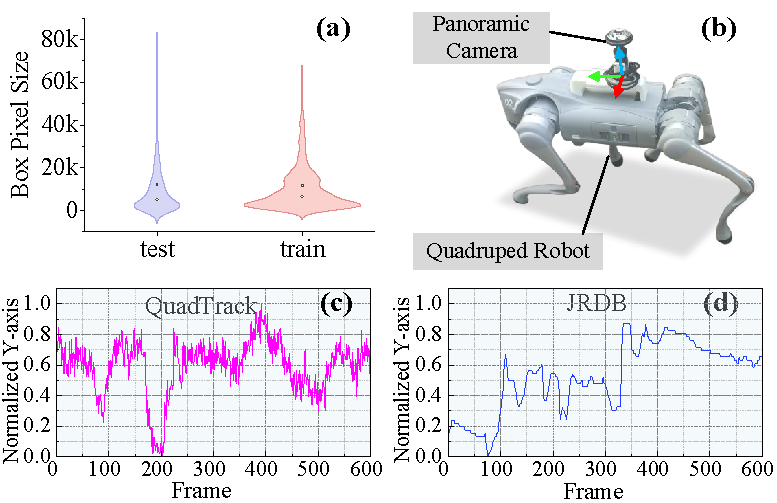
\includegraphics[width=0.48\textwidth]{imgs/robot_plat_v4.pdf}
  \vskip -2ex
  \caption{(a) shows the bounding box (bbox) size distribution for the training and validation sets, whereas (b) depicts the data collection platform and panoramic camera setup. (c) and (d) compare the normalized Y-axis pixel positions of trajectories between the QuadTrack~(\robotdog) and JRDB~\cite{martin2021jrdb}~(\robot) datasets, illustrating the significant vertical motion of the sensor in QuadTrack.}
  \label{fig:robot_platform}
  \vskip -2ex
\end{figure}
\subsection{Data Distribution and Comparative Analysis}
Unlike existing panoramic MOT datasets \cite{milan2016mot16,dendorfer2020mot20,geiger2013vision}, which rely on pinhole cameras, QuadTrack, as shown in Tab.~\ref{tab:comparison dataset}, is the first to be captured using a single $360^{\circ}$ panoramic camera. With a panoramic FoV ($360^{\circ}{\times}70^{\circ}$), QuadTrack significantly differs from traditional MOT datasets \cite{milan2016mot16,dendorfer2020mot20}. In contrast to autonomous driving datasets \cite{caesar2020nuscenes,bdd100k,waymo}, which often feature more predictable motion, QuadTrack incorporates complex, biologically inspired gait movements. Moreover, unlike internet-sourced datasets \cite{peize2021dance,cui2023sportsmot}, QuadTrack is designed to better reflect real-world application scenarios.
While many existing datasets~\cite{vipseg,waymo,caesar2020nuscenes,bdd100k} consist of short video sequences, QuadTrack emphasizes long-term tracking, with each video lasting $60$ seconds. To further challenge data association, we downsampled the dataset to $10$FPS, resulting in $600$ frames per sequence, spread across $32$ sequences. In total, QuadTrack includes $19,200$ frames and $189,876$ bounding boxes. 

%
As illustrated in Fig.~\ref{fig:robot_platform} (a), the distribution of both the training and test sets is consistent, ensuring a reliable and balanced evaluation of MOT methods. This similarity in the distribution between the sets reduces the potential for bias and allows for a more accurate comparison of model performance across varying conditions. The trajectories depicted in Fig.~\ref{fig:robot_platform} (c) and (d) highlight the increased complexity of multi-object tracking under panoramic FoV conditions. Notably, the motion along the Y-axis is significantly more intense compared to JRDB~\cite{martin2021jrdb}, further increasing the difficulty of object detection and association.

\section{Experiments}
\label{sec:experiments}
\begin{figure}
    \centering
    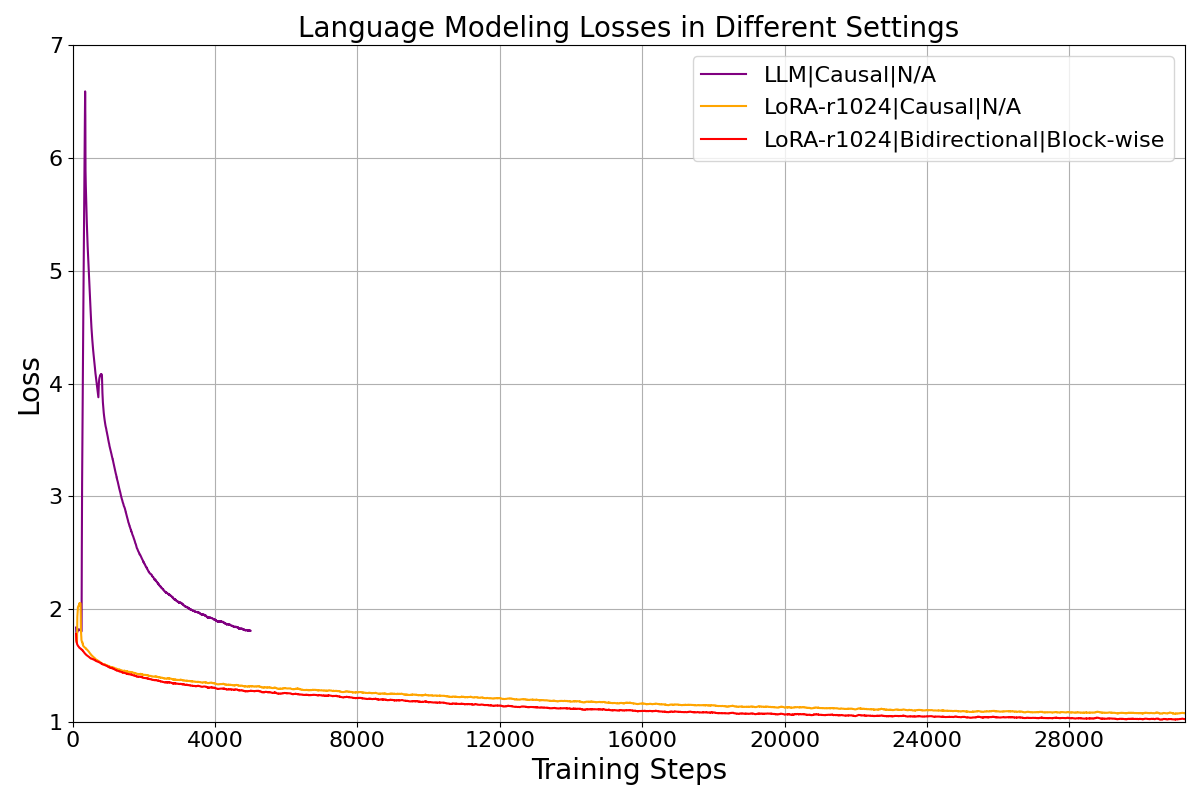
\includegraphics[width=\linewidth]{images/loss_curves_full_llm.png}
    \caption{Language modeling losses in different settings. Training the full LLM with a new modality of data can lead to unrecoverable spike in loss curve, i.e., loss collapse.}
    \label{fig:full_llm}
\end{figure}
\subsection{Implementation details}
\textbf{Training setup.}
Unless otherwise specified, we employed AIMv2-Huge-448p \cite{aimv2} as the default vision encoder and Qwen2.5-7B-Instruct \cite{qwen2.5} as the LLM across all experiments. The pre-training learning rate was fixed at 0.0002 (held constant unless explicitly varied), with 100 warm-up steps and a global batch size maintained at 256. All other hyperparameters and optimizer configurations followed the defaults in \cite{llava1_5}. 

For fine-tuning, all LoRA layers were merged into the LLM, while other components (e.g., distillation modules) were eliminated. The full LLM and 6M-parameter visual embedding layer were trainable. For native-resolution variants (\model{}-AnyRes in Table \ref{tab:ablation}), we retained the pre-trained weights of the fixed-resolution version and adopted native-resolution strategy only during fine-tuning.
\\
\textbf{Benchmarks.} As shown in Table \ref{tab:ablation} and Table \ref{tab:mlm_comparison}, we evaluated the model on several benchmarks: VQAv2: VQAv2 \cite{vqav2}; SQA-I: ScienceQA-Image \cite{scienceqa}; TQA: TextVQA \cite{textvqa}; POPE: POPE \cite{pope}; $\mathrm{MMP_p}$: MME Perception \cite{mme}; $\mathrm{MME_c}$: MME Cognition \cite{mme}; MMB: MMBench \cite{mmbench}; SEED-I: SEED-Image \cite{seed}; MMVet: MMVet \cite{mmvet}; AI2D: AI2D \cite{ai2d}; RQA: Realworld-QA \cite{grok1.5v}; MMMU: MMMU \cite{mmmu}.
% \textbf{Pre-training configurations.} 
% Unless otherwise specified, we employed AIMv2-Huge-448p as our default ViT and Qwen2.5-7B-Instruct as the LLM across all experiments. Detailed hyperparameter settings, including learning rates, batch sizes, and training schedules, were provided in the Appendix.
% \textbf{Visual instruction tuning.} 
% To rigorously evaluate \model{}’s capabilities, we adopted a constrained experimental protocol: using the identical supervised fine-tuning data (LLaVA-665k) and training hyperparameters as LLaVA-1.5 \cite{llava}. This approach enables direct and fair comparison with modular MLLMs and previous monolithic MLLMs \cite{eve, monointernvl} under equivalent data conditions. Our goal is not to outperform via data scaling but to demonstrate that \model{} — despite its monolithic design — achieves performance parity with prevailing modular architectures when given additional pre-training data.
% \textbf{The Setting of ablation studies.} In order to evaluate the impact of key architectural components on visual capability, we curated a subset of 8 million image-text pairs from our DataComp29M-recap dataset.  Text instruction data were excluded from these experiments.
% \textbf{Evaluation Benchmarks.} 
% Our evaluation strategy focuses on two key aspects:
% \begin{itemize}
%     \item \textit{Base Model Capability}: We assess using 10 standard benchmarks: VQAv2, GQA, VizWiz, ScienceQA-Img, TextVQA, POPE, MME, MMBench-EN, Seed-Image, and MM-Vet
%     \item \textit{Ablation Studies}: To accommodate submission limits on VQAv2 and VizWiz, we employ alternative benchmarks for component analysis
% \end{itemize}
% This dual-strategy approach ensures comprehensive validation of \model{}'s core competencies while adhering to platform constraints. All metrics and evaluation protocols align with established practices in multimodal model assessment.
\subsection{Ablation studies}
\begin{figure*}
    \centering
    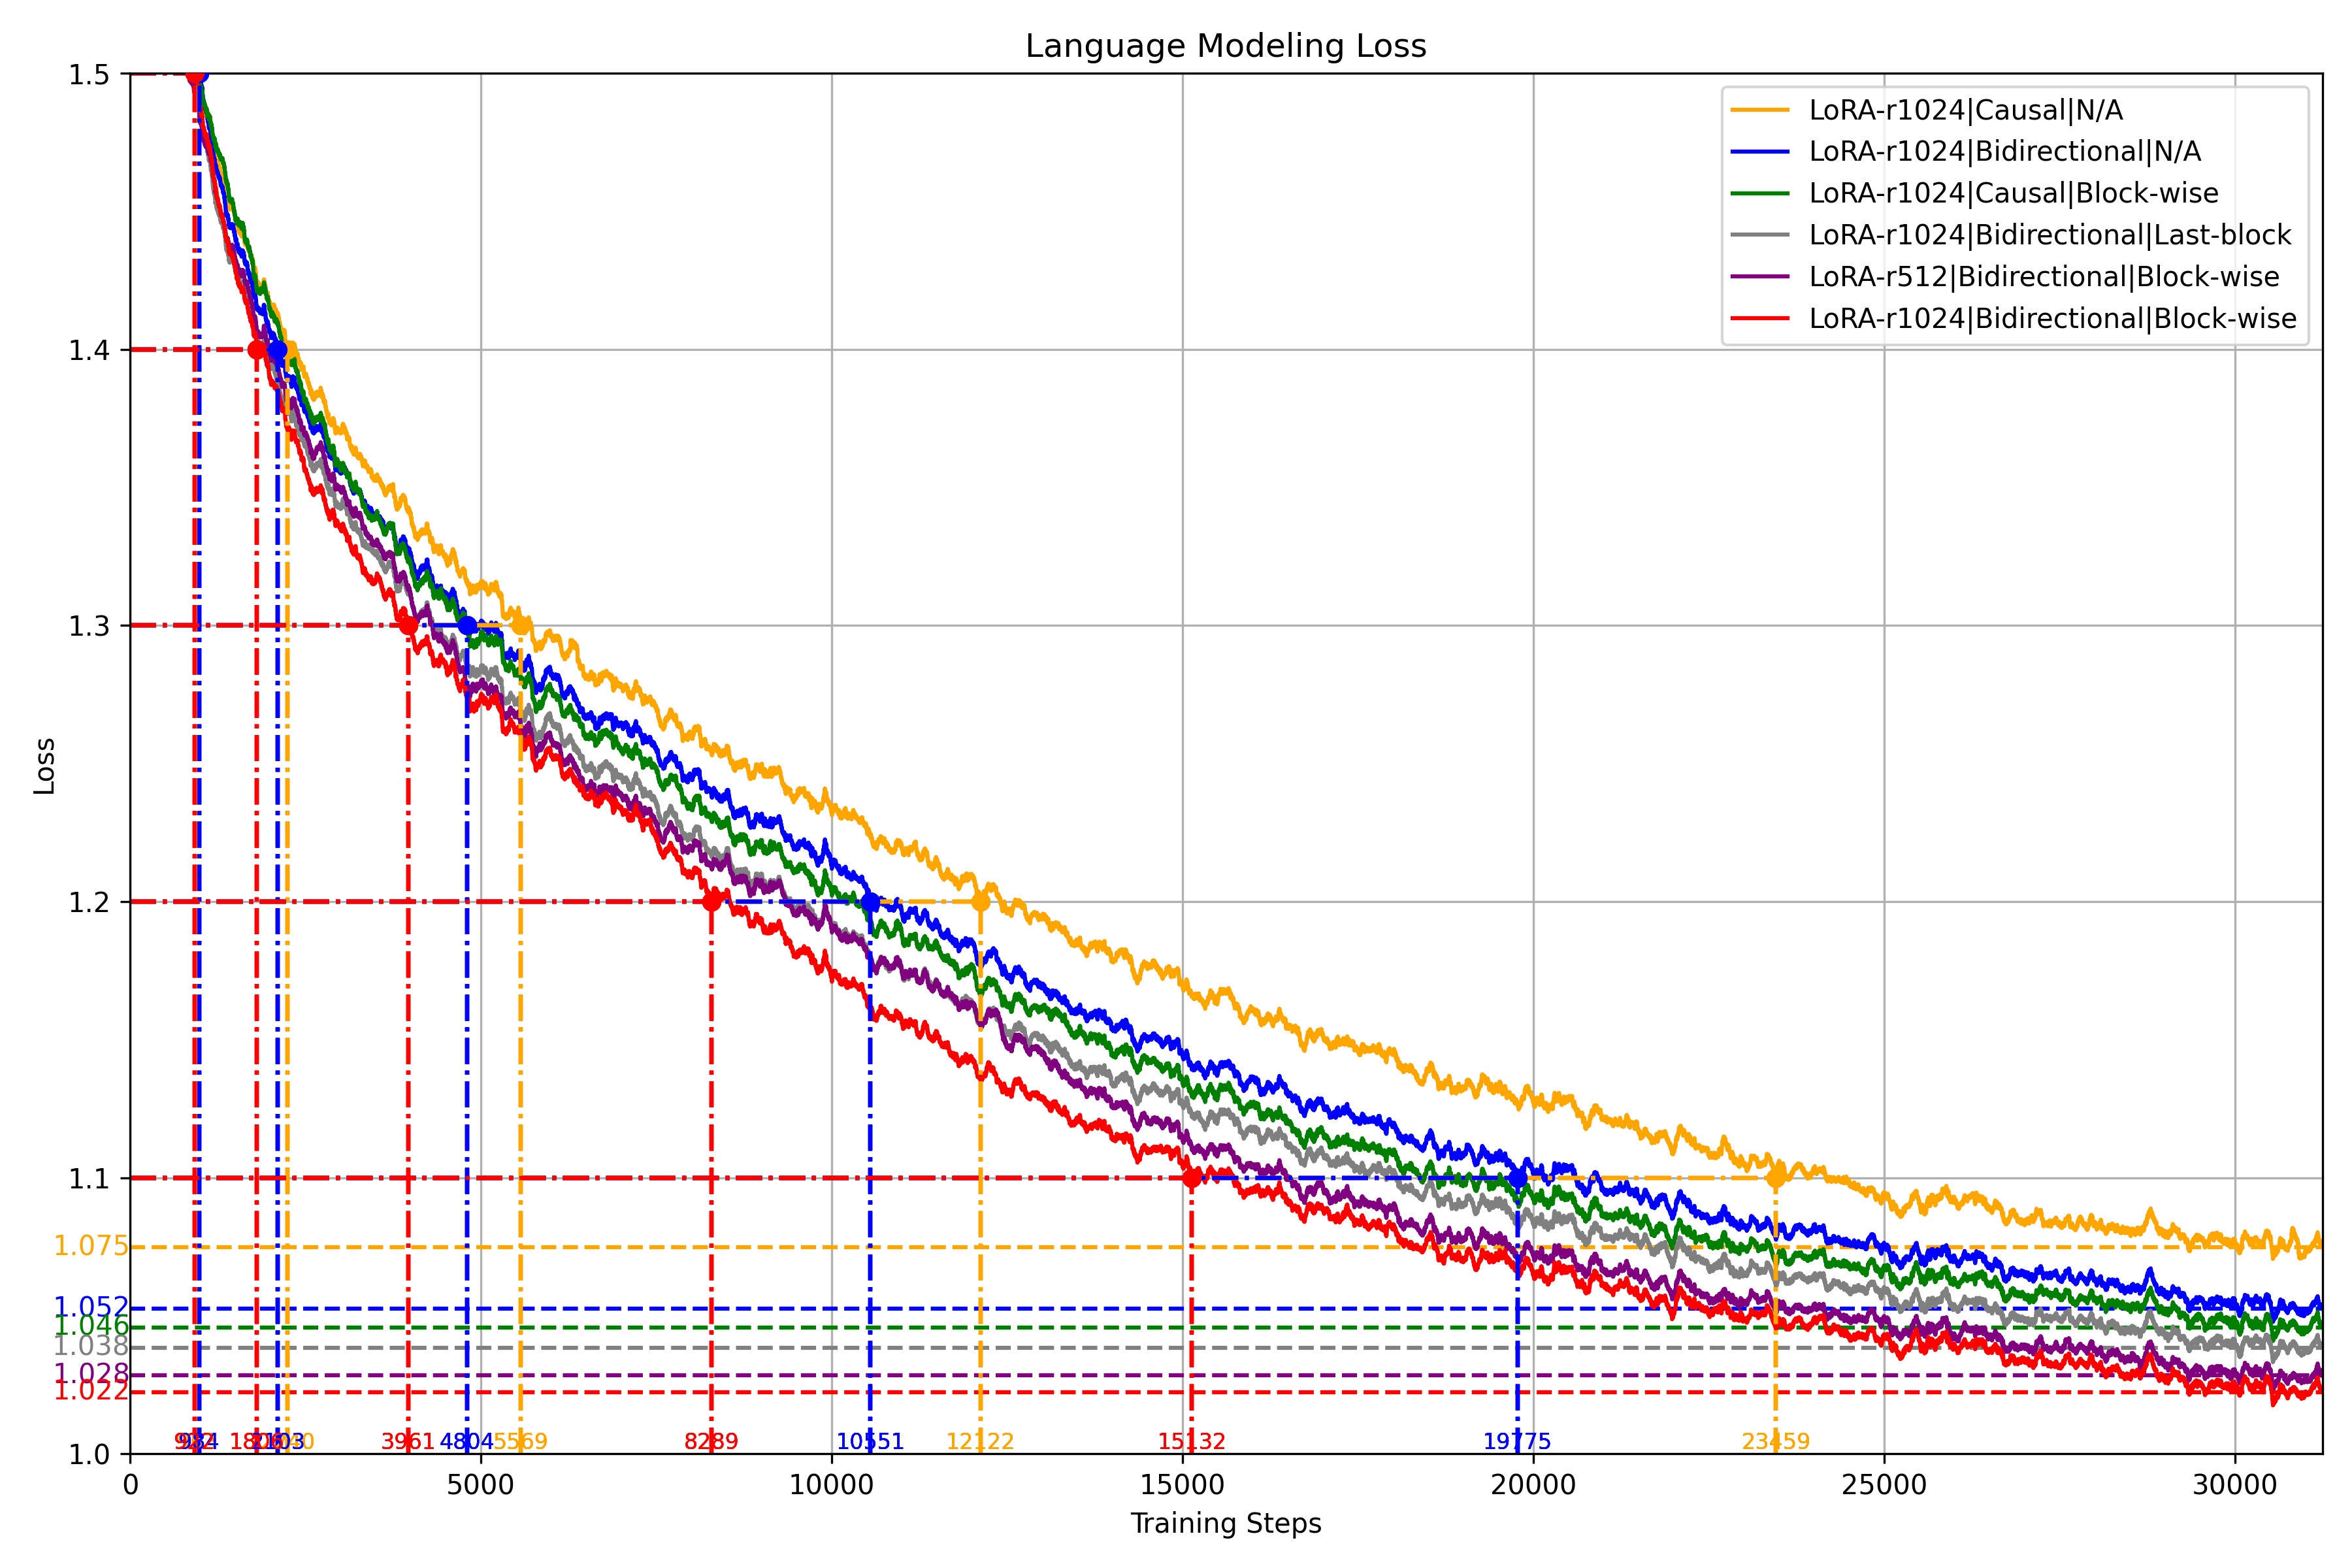
\includegraphics[width=\linewidth]{images/ablation_loss.png}
    \caption{Pre-training loss curves under different configurations. Loss values are smoothed (window=100) for visual clarity. The data sampling order was fixed to ensure fair comparison, as evidenced by the similar trajectories of the loss curves in various settings. LoRA-r1024\textbar Bidirectional\textbar Block-wise refers to the setting: LoRA with rank 1024, bi-directional attention masks for vision, and block-wise distillation. The configuration with the lowest loss was adopted as the default setting in our experiments.}
    \label{fig:ablation_loss}
\end{figure*}
\begin{figure}
    \centering
    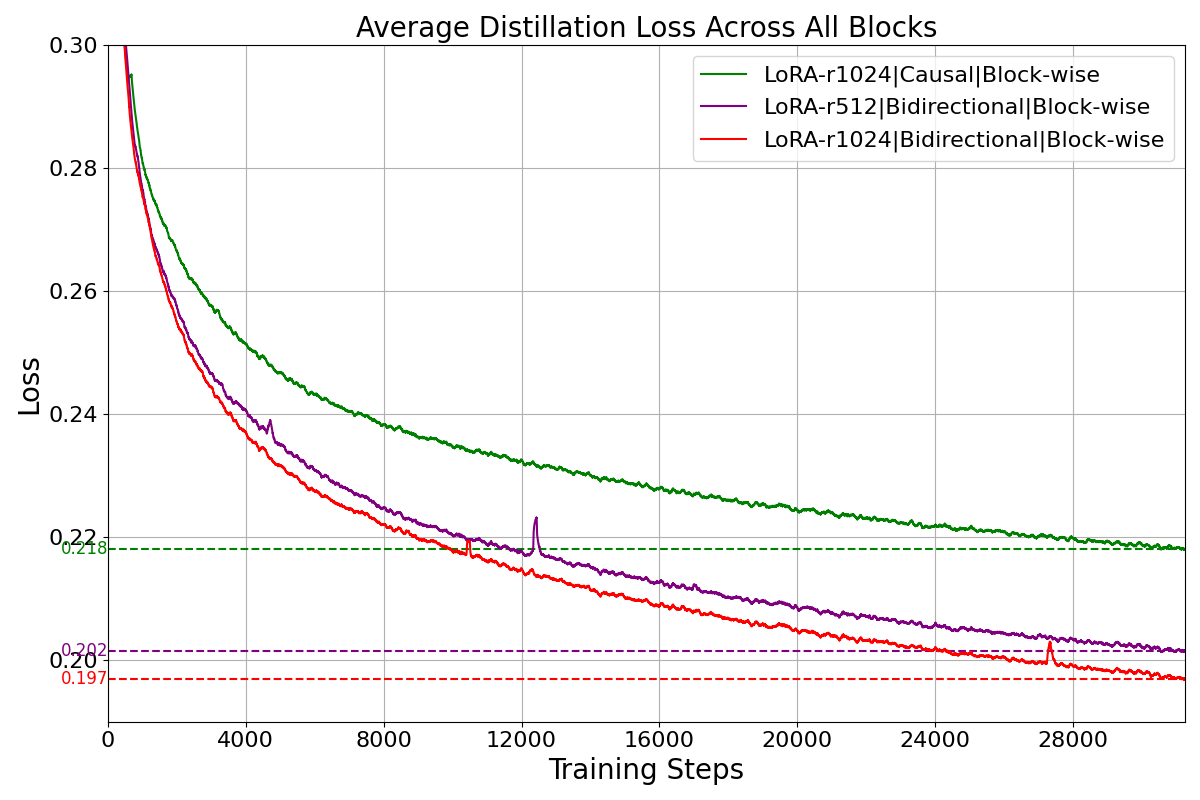
\includegraphics[width=\linewidth]{images/aux_loss_ablation.png}
    \caption{Average distillation loss across all blocks under various settings. Our LoRA-r1024\textbar Bidirectional\textbar Block-wise configuration achieves the lowest average distillation loss across all blocks. This indicates a closer alignment with the ViT’s feature space, confirming that bi-directional attention masks and a larger rank of LoRA layers also enhance visual knowledge transfer.}
    \label{fig:aux_loss}
\end{figure}
% \begin{figure}
%     \centering
%     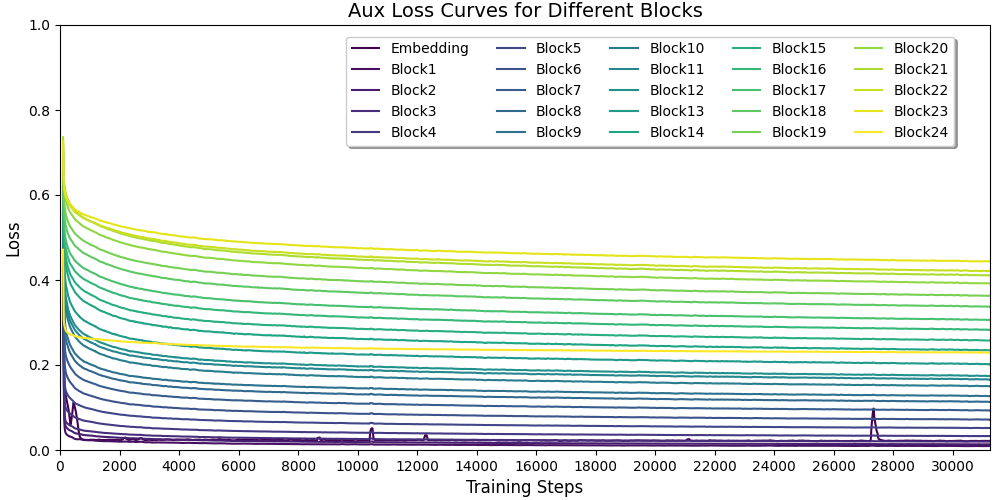
\includegraphics[width=\linewidth]{images/aux_loss.png}
%     \caption{Auxiliary loss for different blocks. loss initially increases with layer depth before declining in later blocks.}
%     \label{fig:aux_loss}
% \end{figure}
\begin{table*}[h]
    \centering
    \renewcommand{\arraystretch}{1.5} % 行间距
    \setlength{\tabcolsep}{3.5pt} % 减少列间距
    \small
    \begin{tabular}{l|c|c|cccccccc|c}
    \toprule
    Vision Params & Visual Attention Mask & Distillation type & TQA & POPE & $\mathrm{MME_p}$ & MMB & SEED-I & MMVet & AI2D & RQA & Avg.\\ 
    \midrule
    % Full LLM (7B) & Causal & N.A. & N.A. & - & - & - & - & - & - & - & - & - \\
    LoRA-r1024 (2B) & Causal & N.A. & 43.7 & 78.6 & 1137.7 & 47.7 & 57.8 & 20.6 & 49.9 & 49.7 & 50.6 \\
    LoRA-r1024 (2B) & Bidirectional & N.A. & 43.6 & 80.9 & 1132.8 & 49.1 & 58.7 & 17.9 & 47.2 & 51.5 & 50.7 \\
    LoRA-r1024 (2B) & Causal & Block-wise & 45.1 & 82.7 & 1172.9 & 52.9 & 63.7 & 20.1 & 50.9 & 51.2 & 53.2 \\
    LoRA-r1024 (2B) & Bidirectional & Last-block & 44.6 & 82.5 & 1197.5 & 51.8 & 63.8 & 17.9 & 49.9 & 52.8 & 52.9 \\
    % LoRA-r1024 (2B) & Bidirectional & Block-wise & AIMv2-Large & - & - & - & - & - & - & - & - & - \\
    LoRA-r512 (1B) & Bidirectional & Block-wise & 47.2 & 83.3 & 1280.5 & 57.6 & 65.3 & 18.5 & 55.9 & 53.1 & 55.6 \\
    % LoRA-r1536 (3B) & Bidirectional & Block-wise & AIMv2-Huge & - & - & - & - & - & - & - & - & - \\
    % LoRA-r1024 (2B) & Bidirectional & Block-wise & Detail & 49.4 & - & - & - & - & - & - & 55.1 & 57.9 \\
    LoRA-r1024 (2B) & Bidirectional & Block-wise & 50.1 & 83.8 & 1224.5 & 53.7 & 65.1 & 22.8 & 52.1 & 55.8 & 55.6 \\
    \bottomrule
    \end{tabular}
    \caption{The performance of various settings on standard benchmarks reveals that lower loss during pre-training correlates with better performance. ``LoRA-r1024 (2B)" indicates that the rank for the LoRA layers is set to 1024, with approximately 2 billion parameters unfrozen for training in total.}
    \label{tab:ablation}
\end{table*}
\begin{figure}
    \centering
    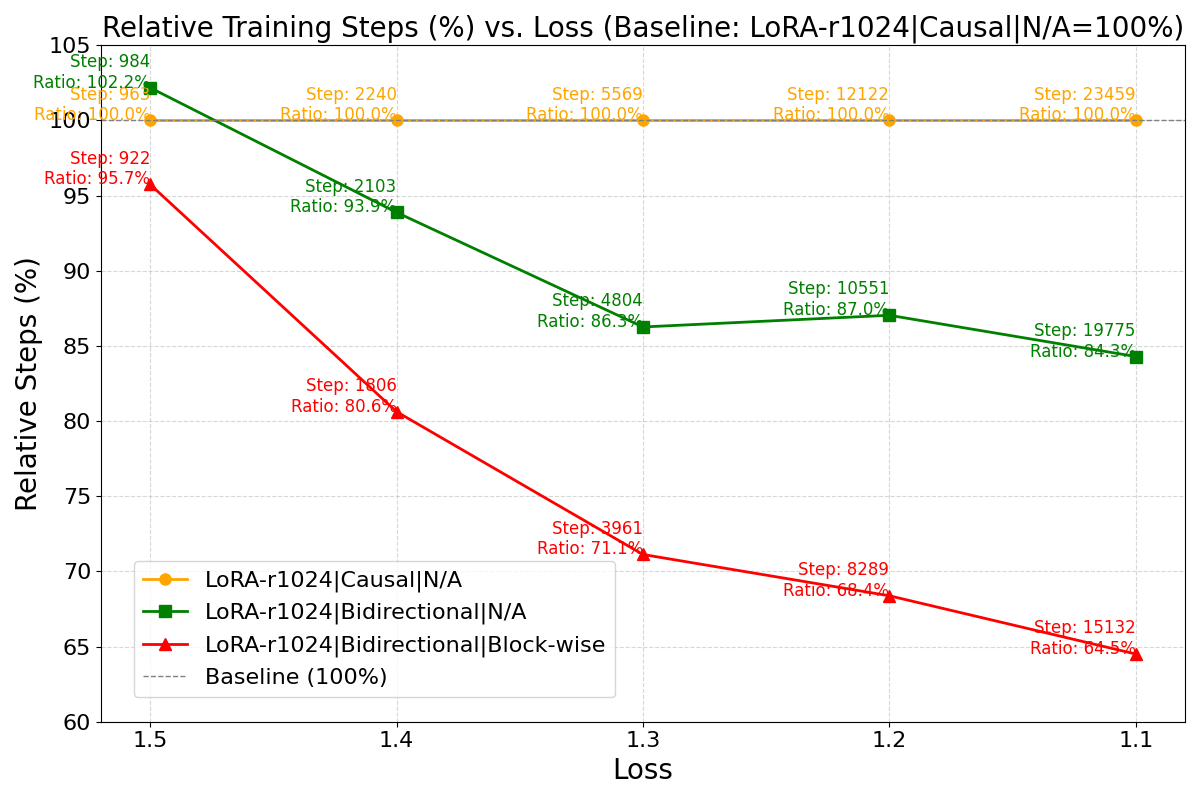
\includegraphics[width=\linewidth]{images/loss_vs_steps.png}
    \caption{Data efficiency analysis. Our experiments demonstrate that combining bi-directional attention masks for vision tokens with block-wise knowledge distillation significantly improves data efficiency compared to the vanilla LoRA configuration. Furthermore, as the target loss decreases (e.g., from 1.5 to 1.1), the required data proportion relative to the baseline diminishes progressively, indicating higher data efficiency.}
    \label{fig:loss_vs_steps}
\end{figure}
Our ablation studies focused on three key components of \model{}: vision as LoRA, block-wise distillation, and bi-directional attention masks for vision. We employed two primary methods to assess performance in various settings: the pre-training loss on an 8M subset of our DataComp29M-recap dataset, as illustrated in Figure \ref{fig:ablation_loss}, and metrics from eight benchmarks, presented in Table \ref{tab:ablation}. Additionally, we visualized the average distillation loss across all blocks, as shown in Figure \ref{fig:aux_loss}.
\\
\textbf{Ablation on vision as LoRA.} Training the full-parameter LLM proved unstable due to modality conflicts (Figure \ref{fig:full_llm}), consistent with findings in \cite{eve}. While reducing the learning rate to a lower value allowed us to observe one successful training case among several attempts, the loss decreased more slowly than that of LoRA-1024. Therefore, we have excluded it from our primary experiments.

Next, we analyzed different LoRA rank configurations in \model{}. Figure \ref{fig:ablation_loss} shows that a rank of 512 resulted in a slightly higher loss (+0.006) compared to rank 1024. This trend continued in the distillation loss (Figure \ref{fig:aux_loss}), where rank 512 showed a modestly higher average block-wise distillation loss (+0.005) compared to rank 1024. Although both configurations ended up with the same average score of 55.6 (Table \ref{tab:ablation}), the consistent loss advantage suggested that higher ranks might have better optimization potential. Furthermore, we experienced training instability with rank 1536, which prompted us to choose rank 1024 as the default configuration.
\\
\textbf{Ablation on bi-directional attention masks.} 
As demonstrated in Figure~\ref{fig:ablation_loss}, under fixed hyperparameters (e.g., LoRA rank and distillation type), the bi-directional attention mask consistently achieved lower training loss compared to causal masking. This empirical advantage was further supported by the reduced average distillation loss across all Transformer blocks, as depicted in Figure~\ref{fig:aux_loss}. Quantitatively, as evidenced in Table~\ref{tab:ablation}, replacing causal masking with bi-directional masks yielded significant performance improvements. For instance, switching from LoRA-r1024\textbar Causal\textbar Block-wise to LoRA-r1024\textbar Bidirectional\textbar Block-wise led to a 2.4-point average score gain, while replacing LoRA-r1024\textbar Causal\textbar N/A with LoRA-r1024\textbar Bidirectional\textbar N/A yielded a gain of 0.1 points.  
\\
\textbf{Block-wise distillation.} As shown in Figure~\ref{fig:ablation_loss} and Table~\ref{tab:ablation}, applying distillation to the final Transformer block alone significantly improved training efficiency. For example, the transition from the configuration LoRA-r1024\textbar{}Bidirectional\textbar{}N/A to LoRA-r1024\textbar{}Bidirectional\textbar{} Last-block yielded a 2.7-point score gain and a 0.016 reduction in loss. Extending distillation to all blocks via block-wise supervision further enhanced performance: compared with LoRA-r1024\textbar{}Bidirectional\textbar{}Last-block, LoRA-r1024\textbar{}Bidirectional\textbar{}Block-wise produced an additional 2.7-point gain and 0.016 loss reduction. These results indicated that the vanilla distillation method, i.e., last-block distillation, could accelerate training, and block-wise distillation could even strengthen this effect.
\\
% \textbf{Data strategy.} We also examined the impact of using detailed versus standard caption data during the early training stage. As shown in Table \ref{tab:ablation}, employing detailed captions for early-stage pre-training was suboptimal compared to using standard captions. This might be due to the rich and intricate visual clues present in the detailed captions, which could be too fine-grained for a model lacking prior visual capabilities to effectively learn from.
% \\
\textbf{Data efficiency analysis.} We measured data efficiency by reporting the relative number of training steps required to reach certain loss thresholds, using vanilla LoRA as the baseline. 

As illustrated in Figure~\ref{fig:loss_vs_steps}, the bi-directional attention variant without distillation (LoRA-r1024\textbar{}Bidirectional\textbar{}N/A) required 102.2\% of the baseline training steps to reach Loss=1.5, whereas adding block-wise distillation (LoRA-r1024\textbar{}Bidirectional\textbar{}Block-wise) reduced this to 95.7\%. The efficiency gap became more pronounced at lower loss: at Loss=1.1, the same configurations needed 84.3\% and 64.5\% of the vanilla LoRA baseline steps, respectively. This demonstrated that our optimal configuration achieved equivalent convergence with 35.5\% fewer training steps than vanilla LoRA.

Furthermore, the ratio of data needed by our best configuration relative to vanilla LoRA decreased over time, implying that comparable performance could be achieved with $N\times$ fewer training data.
\subsection{Standard evaluation}
\begin{table*}[h]
    \centering
    \renewcommand{\arraystretch}{1.5} % 减少行间距
    \setlength{\tabcolsep}{0.6pt} % 减少列间距
    \footnotesize % 或者使用 \footnotesize
    \begin{tabular}{llccccccccccccccccc}
        \toprule
        \multirow{2}{*}{Method} & \multirow{2}{*}{LLM} & \multirow{2}{*}{ViT} & \multicolumn{2}{c}{\# Sample} & \multirow{2}{*}{VQAv2} & \multirow{2}{*}{SQA-I} & \multirow{2}{*}{TQA} & \multirow{2}{*}{POPE} & \multirow{2}{*}{$\mathrm{MME_p}$} & \multirow{2}{*}{$\mathrm{MME_c}$} & \multirow{2}{*}{MMB} & \multirow{2}{*}{SEED-I} & \multirow{2}{*}{MMVet} & \multirow{2}{*}{AI2D} & \multirow{2}{*}{RQA} & \multirow{2}{*}{MMMU}\\
        \cmidrule{4-5}
        & & & Pretrain & Finetune & & & & & & & & & & \\
        \midrule
        % 在这里添加数据行
        \textit{Encoder-based}\\
        \midrule
        \rowcolor{gray!30}  
        BLIP2 \cite{blip2} & Vicuna-13B & EVA-1B & 129M & - & 65.0 & 61 & 42.5 & 85.3 & 1293.8 & - & - & 49.7 & 22.4 & - & - & - \\
        \rowcolor{gray!30}  
        InstructBLIP \cite{instructblip} & Vicuna-7B & EVA-1B & 129M & 1.2M & - & 60.5 & 50.1 & - & - & - & 36 & 58.8 & 26.2 & - & - & - \\
        \rowcolor{gray!30}  
        InstructBLIP \cite{instructblip} & Vicuna-13B & EVA-1B & 129M & 1.2M & - & 63.1 & 50.7 & 78.9 & 1212.8 & - & - & - & 25.6 & - & - & - \\
        LLaVA-1.5 \cite{llava1_5} & Vicuna-7B & CLIP-0.3B & 558K & 665K & 78.5 & 66.8 & 58.2 & 85.9 & 1510.7 & 316.1 & 64.3 & 66.1 & 31.1 & 54.8 & 54.8 & 35.3\\
        % LLaVA-1.5 \cite{aimv2} & Vicuna-7B & AIMv2-0.3B & 8M & 665K & vqav2 & sqa-i & tqa & pope & mmep & mmec & mmb & seed-i & mmvet & ai2d & rqa & mmmu\\
        LLaVA-1.5 \cite{llava1_5} & Qwen2.5-7B & AIMv2-0.6B & 558K & 665K & 82.3 & 77.5 & 59.2 & 85.2 & 1582.3 & 313.0 & 66.3 & 70.6 & 33.7 & 63.7 & 60.0 & 35.3\\
        \midrule
        \textit{Encoder-free}\\
        \midrule
        % \model{} & Qwen2.5-7B & \sout{AIMv2-0.6B} & 8M & 665K & vqav2 & sqa-i & tqa & pope & mmep & mmec & mmb & seed-i & mmvet & ai2d & rqa & mmmu\\
        % \model{} & Qwen2.5-7B & \sout{AIMv2-0.6B} & 8M & 665K & vqav2 & sqa-i & 50.1 & 83.8 & 1224.5 & 274.6 & 53.7 & 65.1 & 22.8 & 52.1 & 55.8 & \\
        \model{} & Qwen2.5-7B & \sout{AIMv2-0.6B} & 30M & 665K & 76.0 & 75.9 & 56.3 & 84.5 & 1363.4 & 311.1 & 64.2 & 67.5 & 33.7 & 65.6 & 57.7 & 32.2\\
       \model{}-AnyRes & Qwen2.5-7B & \sout{AIMv2-0.6B} & 30M & 665K & 76.0 & 72.0 & 58.7 & 85.5 & 1336.1 & 319.3 & 61.3 & 68.9 & 33.7 & 61.1 & 60.1 & 32.0\\
       EVE \cite{eve} & Vicuna-7B & \sout{CLIP-0.3B} & 49M(2) & 665K & 75.4 & 63.0 & 51.9 & 83.6 & 1217.3 & 266 & 49.5 & 61.3 & 25.6 & 48.5 & - & - \\
   \rowcolor{gray!30} 
      EVE-HD \cite{eve} & Vicuna-7B & \sout{CLIP-0.3B} & 49M(2) & 1.8M & 74.2 & 64.9 & 56.8 & 85.0 & 1305.7 & 322 & 52.3 & 64.6 & 25.7 & 61.0 & - & - \\
    \rowcolor{gray!30}  
      EVEv2 \cite{evev2} & Qwen2.5-7B & - & 87M(2) & 22.3M(2) & - & 96.2 & 71.1 & 87.6 & - & - & 66.3 & 71.4 & 45.0 & 74.8 & 62.4 & 39.3 \\
  \rowcolor{gray!30}  
      Mono-InternVL \cite{monointernvl} & Intern1.5-2B & - & 1.2B(2) & 150M(2) & - & 93.6 & 72.6 & - & - & - & 65.5 & 67.4 & 40.1 & 68.6 & - & 33.7 \\
      Mono-InternVL \cite{monointernvl} & Intern1.5-2B & - & 922M & 665K & - & 57 & 49 & - & 1100 & - & - & - & - & 42 & - & - \\
    Mono-InternVL \cite{monointernvl} & Intern1.5-2B & - & 1.2B(2) & 665K & - & 58 & 55 & - & 1110 & - & - & - & - & 46 & - & - \\
        \bottomrule
    \end{tabular}
    \caption{Comparison with previous methods on several benchmarks. Since this paper aims to demonstrate that \model{} is a strong base model, we did not scale the fine-tuning data. Therefore, we did not compare with recent state-of-the-art models that often require additional data engineering or involve proprietary datasets; methods that utilize extra fine-tuning data are grayed out. We classified domain-specific VQA data as fine-tuning data rather than pre-training data for EVEv2 and Mono-InternVL, which differs from their original classification in the respective papers. The notation ``49M(2)" indicates that this method employs a two-stage training process using a total of 49M image-text pairs. The strikethrough notation \sout{ViT} means that ViT is excluded during inference.}
    \label{tab:mlm_comparison}
\end{table*}
To ensure a fair comparison between \model{} and existing methods, we deliberately restricted our experimental design. While prior works (e.g., EVE, EVEv2 \cite{evev2}, and Mono-InternVL \cite{monointernvl}) have leveraged massive in-domain datasets (Table~\ref{tab:mlm_comparison}), such approaches complicated direct comparisons due to proprietary training data. Our goal is not to pursue state-of-the-art performance on benchmarks but to validate a novel MLLM architecture. Thus, we limited fine-tuning to the publicly available LLaVA-665K dataset without additional scaling.

To eliminate the potential advantages provided by LLMs and ViTs, we also trained a LLaVA-1.5 model using Qwen-2.5-7B and AIMv2-0.6B. As shown in Table~\ref{tab:mlm_comparison}, prior encoder-free methods often adopted intricate multi-stage pipelines involving module freezing strategies and proprietary datasets (e.g., 100M–1.2B samples). In contrast, our framework employed a streamlined single-stage training process (pre-training followed by fine-tuning), using about 30M image-text pairs. 
% In contrast to the claims made in EVEv2 \cite{evev2} and Mono-InternVL \cite{monointernvl}, we classified domain-specific VQA data in Table \ref{tab:mlm_comparison} as fine-tuning data rather than pre-training data, aligning with the community's consensus. 

As shown in Table~\ref{tab:mlm_comparison}, \model{} achieved performance comparable to both official and reproduced LLaVA-1.5 baselines on most benchmarks when evaluated under strict LLaVA-1.5 protocols \cite{llava1_5}, i.e., identical prompts/generation parameters. However, \model{} underperformed on MME Perception, a gap we attribute to limited world knowledge in our pre-training data. This was further quantified in Table~\ref{tab:world_knowledge}, where \model{} struggled with tasks demanding intensive world-knowledge: 1) inferring movie details from posters, 2) identifying celebrities, 3) recognizing landmarks, and 4) classifying artworks, as these tasks required external domain knowledge absent in our training datasets.

\begin{table}[]
    \centering
    \renewcommand{\arraystretch}{1.5}
    \small
    \setlength{\tabcolsep}{3pt}
    \begin{tabular}{c|cccc|c}
    \toprule
        Method & Posters & Celebrity & Landmark & Artwork & Total\\
        \midrule
        LLaVA-1.5 & 156.1 & 143.5 & 173.5 & 134.0 & 607.1\\
        \midrule
        VoRA & 117.3 & 111.2 & 139.3 & 105.5 & 473.3\\
        VoRA-AnyRes & 110.2 & 104.7 & 138.0 & 110.8 & 463.7\\
    \bottomrule
    \end{tabular}
    \caption{The performance of VoRA in world knowledge tasks. We acknowledge its deficiency, as expected, due to the lack of relevant in-domain data in our pre-training dataset. This is the primary reason for our lower performance on the MME Perception benchmark.}
    \label{tab:world_knowledge}
\end{table}
\section{Conclusion}
\label{sec:Conclusion}
%
This paper presents OmniTrack, a multi-object tracking framework tailored for panoramic images, effectively addressing key challenges like geometric distortion, low resolution, and lighting inconsistencies. Central to OmniTrack is a feedback mechanism that reduces uncertainty in panoramic-FoV tracking. The framework incorporates Tracklets Management for temporal stability, FlexiTrack Instance for rapid localization and association, and the CircularStatE Module to mitigate distortion and improve visual consistency.
%
Additionally, we present QuadTrack, a cross-campus multi-object tracking dataset collected using a quadruped robot to support dynamic motion scenarios. 
This challenging dataset is designed to advance research in omnidirectional perception for robotics. Experiments verify that OmniTrack achieves state-of-the-art performance on public JRDB and the established QuadTrack datasets, demonstrating its effectiveness in handling panoramic tracking tasks.


\noindent\textbf{Limitations.} 
%
While OmniTrack demonstrates strong performance, our approach is currently limited to 2D panoramic tracking without 3D capabilities, restricting depth perception in complex scenes. Additionally, the method is centered around a mobile robotic platform. Future work could consider extending to 3D panoramic MOT or exploring human-robot collaborative perception to enhance situational awareness.


\section*{Acknowledgment}
\label{sec:Acknowledgment}
This work was supported in part by the National Natural Science Foundation of China (No.~62473139 and No.~12174341), in part by Zhejiang Provincial Natural Science Foundation of China (Grant No. LZ24F050003), and in part by Shanghai SUPREMIND Technology Co. Ltd.


% \clearpage
{
    \small
    \bibliographystyle{ieeenat_fullname}
    \bibliography{main}
}

\clearpage
\appendix
\setcounter{page}{1}
\maketitlesupplementary

\section{Implementation Details}
We follow prior studies\cite{coop, cocoop, prograd, kgcoop, maple, tcp, mma} and adopt a 16-shot learning setting across all experiments, except for the few-shot learning tasks. The ViT-B/16\cite{vit} variant of the CLIP model serves as the visual backbone for all experimental setups. Hand-crafted text prompts from prior methods\cite{clip, coop, tip-adapter} are utilized and described in detail in \cref{datasets}. Optimization is performed using the AdamW optimizer with an initial learning rate of 0.001. All our models are trained with mix-precision for speeding up. For the larger ImageNet dataset, we employ a batch size of 32, while a batch size of 4 is used for all other datasets. Training on ImageNet for the base-to-novel generalization task spans 5 epochs, whereas training on the remaining datasets is conducted over 10 epochs. For cross-dataset evaluation and domain generalization tasks, we perform training for a single epoch on ImageNet. In the few-shot learning tasks, training is carried out for 5 epochs on ImageNet and 50 epochs for other datasets. The average accuracy is reported over three independent runs, with all experiments executed on a single NVIDIA RTX 4090 GPU.

Representation tokens are initialized from a zero-mean Gaussian distribution with a standard deviation of 0.02. We set $J = 6$, integrating the representation tokens beginning at the 6-th transformer layer. The dimension of the representation space, $d_r$, is set to 2048 for EuroSAT and 512 for all other datasets. Note that since the $d_r$ setting for EuroSAT differs from other datasets, in the $d_r$ ablation experiments we fix $d_r$ for EuroSAT to 2048 while adjusting $d_r$ on the other datasets. The number of representation tokens, $K$, is configured to 5. The parameter $\alpha$ is fixed at 0.7, and the details regarding the configuration of $\lambda$ are provided in \cref{ablation_lambda}.



\section{Dataset Details}
Details of 14 datasets are shown in \cref{datasets}.


\section{Computational Cost}
Table \ref{computational_cost} summarizes the learnable parameters, training time per image, total training duration, inference speed (measured in frames per second, FPS, with a batch size of 100), and the final HM metric for each approach. Our proposed model, MMRL, demonstrates a compelling balance of computational efficiency and performance. The key observations are as follows:
\begin{itemize}
    \item Models incorporating multimodal interaction mechanisms (e.g., MaPLe, MMA, and MMRL) generally involve a higher parameter count compared to models without such mechanisms.
    \item Both MMRL and the prior MMA approach exhibit significantly faster training speed, thereby reducing overall computational costs. While MaPLe and PromptSRC achieve higher inference speeds, their training durations are relatively longer. Notably, MMRL offers faster inference compared to MMA and MetaPrompt.
    \item To assess the performance of MMRL under constrained computational resources, we reduced the dimensionality of the representation space from 512 to 32. In this configuration, MMRL achieves a parameter count comparable to that of MMA, while still significantly outperforming the previous state-of-the-art model.
\end{itemize}



\begin{table}[h]
\centering
\renewcommand\arraystretch{1.25}
\caption{All methods were trained on a single NVIDIA RTX 4090 GPU using the ImageNet dataset. Each model was implemented with publicly available code and default configurations as described in their respective papers \cite{maple, promptsrc, provp, metaprompt, tcp, mma}. `V-L' denotes vision-language interaction, indicating that efficient fine-tuning incorporates interactions between visual and textual modalities before prediction. `V, L' signifies separate fine-tuning of each modality without inter-modal interaction before prediction, while `L' refers to fine-tuning limited to the textual modality alone. `Train time' is reported as both time per image and the total duration for training the full dataset(16-shots), while `FPS (100 BS)' indicates frames per second with a batch size of 100 during inference.}
\label{computational_cost}
\resizebox{0.475\textwidth}{!}{
    \begin{tabular}{@{}l|ccccc|c@{}}
    \toprule
    \multirow{2}{*}{Method} & \multirow{2}{*}{Modality} & Params & Train time & Train time & FPS & \multirow{2}{*}{HM} \\
               &     & (learnable) & (ms/image) & (minute/all) & (100 BS) &       \\ \midrule
    MaPLe      & V-L & 3.555M      & 39.5       & 26.4         & 1757.6   & 78.55 \\
    PromptSRC  & V,L & 0.046M      & 40.0       & 106.8        & 1764.2   & 79.97 \\
    ProVP      & V   & 0.147M      & 4.4        & 107.2        & 928.9    & 78.76 \\
    MetaPrompt & V,L & 0.031M      & 30.7       & 32.8         & 659.8    & 79.09 \\
    TCP        & L   & 0.332M      & 5.3        & 17.7         & 950.6    & 79.51 \\
    MMA        & V-L & 0.675M      & 2.2        & 1.5          & 688.5    & 79.87 \\ \midrule
    MMRL       & V-L & 4.992M      & 5.3        & 3.6          & 762.4    & 81.20 \\
    MMRL*      & V-L & 0.689M      & 5.3        & 3.6          & 767.8    & 80.84 \\ \bottomrule
    \end{tabular}
}
\end{table}


\section{Ablation Analysis on $\lambda$}
As shown in \cref{ablation_lambda}, increasing the value of $\lambda$ generally improves performance, with the optimal or near-optimal results typically observed when $\lambda$ is set between 4 and 6 across most datasets. Notably, as $\lambda$ continues to increase, its impact on model performance within the same dataset diminishes, indicating reduced sensitivity to variations in $\lambda$. This trend suggests that the model becomes more robust and less reliant on precise tuning of $\lambda$ at higher values.


\begin{table*}[h]
\centering
\caption{Summary of the 14 datasets.}
\label{datasets}
\renewcommand\arraystretch{1.2}
\resizebox{1.0\textwidth}{!}{
    \begin{tabular}{@{}l|llllll@{}}
    \toprule
    Dataset      & Classes & Train  & Val    & Test   & Description                         & Prompt                                \\ \midrule
    ImageNet     & 1000    & 1.28M  & $\sim$ & 50000  & Recognition of generic objects      & ``a photo of a [CLASS].”              \\
    Caltech101   & 100     & 4128   & 1649   & 2465   & Recognition of generic objects      & ``a photo of a [CLASS].”              \\
    OxfordPets      & 37    & 2944   & 736    & 3669   & Fine-grained classification of pets                    & ``a photo of a [CLASS], a type of pet.”      \\
    StanfordCars & 196     & 6509   & 1635   & 8041   & Fine-grained classification of cars & ``a photo of a [CLASS].”              \\
    Flowers102      & 102   & 4093   & 1633   & 2463   & Fine-grained classification of flowers                 & ``a photo of a [CLASS], a type of flower.”   \\
    Food101         & 101   & 50500  & 20200  & 30300  & Fine-grained classification of foods                   & ``a photo of [CLASS], a type of food.”       \\
    FGVCAircraft    & 100   & 3334   & 3333   & 3333   & Fine-grained classification of aircrafts               & ``a photo of a [CLASS], a type of aircraft.” \\
    SUN397       & 397     & 15880  & 3970   & 19850  & Scene classification                & ``a photo of a [CLASS].”              \\
    DTD          & 47      & 2820   & 1128   & 1692   & Texture classification              & ``[CLASS] texture.”                   \\
    EuroSAT         & 10    & 13500  & 5400   & 8100   & Land use \& cover classification with satellite images & ``a centered satellite photo of [CLASS].”    \\
    UCF101       & 101     & 7639   & 1898   & 3783   & Action recognition                  & ``a photo of a person doing [CLASS].” \\ \midrule
    ImageNetV2   & 1,000   & $\sim$ & $\sim$ & 10,000 & New test data for ImageNet          & ``a photo of a [CLASS].”              \\
    ImageNet-Sketch & 1,000 & $\sim$ & $\sim$ & 50,889 & Sketch-style images of ImageNet classes                & ``a photo of a [CLASS].”                     \\
    ImageNet-A      & 200   & $\sim$ & $\sim$ & 7,500  & Natural adversarial examples of 200 ImageNet classes   & ``a photo of a [CLASS].”                     \\
    ImageNet-R   & 200     & $\sim$ & $\sim$ & 30,000 & Renditions of 200 ImageNet classes  & ``a photo of a [CLASS].”              \\ \bottomrule
    \end{tabular}
    }
\end{table*}


\begin{table*}[h]
\centering
\caption{Ablation on $\lambda$ across 11 datasets, with results evaluated using the harmonic mean (HM) metric.}
\label{ablation_lambda}
\renewcommand\arraystretch{1.2}
\resizebox{1.0\textwidth}{!}{
    \begin{tabular}{@{}c|ccccccccccc@{}}
    \toprule
    $\alpha$ & ImageNet       & Caltech101     & OxfordPets & StanfordCars & Flowers102 & Food101 & FGVCAircraft   & SUN397         & DTD            & EuroSAT & UCF101 \\ \midrule
    0.0  & 74.01 & 95.97 & 96.35          & 76.00          & 84.42          & 90.10          & 38.52 & 79.67 & 68.21 & 82.65          & 81.63          \\
    0.01 & 74.07 & 96.12 & 96.39          & 75.95          & 84.82          & 90.23          & 37.87 & 79.85 & 67.73 & \textbf{87.21} & 82.11          \\
    0.1  & 74.23 & 96.25 & 96.49          & 76.32          & 84.81          & 90.53          & 38.66 & 80.23 & 69.79 & 83.21          & 82.91          \\
    0.2  & 74.38 & 96.40 & \textbf{96.74} & 76.67          & 85.31          & 90.61          & 39.27 & 80.25 & 70.58 & 82.68          & 82.70          \\
    0.5      & \textbf{74.45} & \textbf{96.68} & 96.54      & 77.09        & 85.74      & 90.86   & 40.37          & 80.61          & 72.67          & 82.87   & 83.05  \\
    3.0  & 74.09 & 96.59 & 96.51          & 77.72          & 86.65          & 90.98          & 40.48 & 81.10 & 73.54 & 77.95          & \textbf{83.89} \\
    4.0  & 74.04 & 96.62 & 96.55          & 77.73          & \textbf{86.78} & 90.98          & 40.66 & 81.14 & 73.75 & 77.27          & 83.45          \\
    5.0  & 73.93 & 96.62 & 96.60          & 77.86          & 86.42          & \textbf{91.03} & 40.42 & 81.07 & 73.69 & 78.05          & 83.84          \\
    6.0      & 73.83          & 96.61          & 96.66      & 78.05        & 86.48      & 91.00   & \textbf{41.15} & \textbf{81.20} & \textbf{73.82} & 75.23   & 83.68  \\
    7.0  & 73.78 & 96.62 & 96.58          & \textbf{78.06} & 86.53          & 90.95          & 40.88 & 81.10 & 73.65 & 75.85          & 83.55          \\
    10.0 & 73.68 & 96.64 & 96.56          & 77.86          & 86.46          & 91.00          & 41.01 & 80.93 & 73.68 & 77.61          & 83.38          \\ \bottomrule
    \end{tabular}
}
\end{table*}

\begin{table}[t]
\small
\centering
\caption{Ablation on different regularization strategies.}
\label{ablation_regularization}
\begin{tabular}{@{}c|ccc@{}}
\toprule
Regularization & Base           & Novel          & HM             \\ \midrule
\rowcolor[HTML]{EFEFEF} 
Cosine         & \textbf{85.68} & \textbf{77.16} & \textbf{81.20} \\
L1             & 85.46          & 76.03          & 80.47          \\
MSE             & 85.13          & 74.62          & 79.53          \\ \bottomrule
\end{tabular}
\end{table}

\section{Ablation Analysis on Regularization Strategies}
We investigate the impact of various regularization strategies aimed at maximizing the similarity between class token features and frozen CLIP features to retain pre-trained knowledge. The results, summarized in \cref{ablation_regularization}, indicate that cosine regularization achieves the best performance. In contrast, both L1 and MSE losses lead to performance degradation, with MSE causing a significant decline. This result can be attributed to the more relaxed and flexible constraints of cosine regularization, enabling the class token to preserve generalizability while effectively capturing task-specific knowledge.






\section{Few-Shot Learning}
\cref{few_shot1,few_shot2} provide detailed comparisons of MMRL and prior state-of-the-art methods on few-shot learning across 11 datasets. MMRL achieves the highest average performance across all shots. Note that the MMA results are reproduced from the open-source code, as the original paper does not report results for this experiment.







\begin{table*}[t]
\small
\centering
\caption{Comparison of MMRL with previous state-of-the-art methods on few-shot learning across 11 datasets.}
\label{few_shot1}
\setlength{\tabcolsep}{15pt}{
\resizebox{0.9\textwidth}{!}{
    \begin{tabular}{@{}ll|ccccc}
    \toprule
    \textbf{Dataset} &
      \textbf{Method} &
      \textbf{1 shot} &
      \textbf{2 shots} &
      \textbf{4 shots} &
      \textbf{8 shots} &
      \textbf{16 shots} \\ \midrule
     &
      Linear probe CLIP &
      45.83 &
      57.98 &
      68.01 &
      74.47 &
      78.79 \\
     &
      CoOp &
      67.56 &
      70.65 &
      74.02 &
      76.98 &
      79.89 \\
     &
      CoCoOp &
      66.79 &
      67.65 &
      71.21 &
      72.96 &
      74.90 \\
     &
      MaPLe &
      69.27 &
      72.58 &
      75.37 &
      78.89 &
      81.79 \\
     &
      PromptSRC &
      72.32 &
      75.29 &
      78.35 &
      80.69 &
      82.87 \\
     &
      MMA &
      69.28 &
      72.08 &
      76.38 &
      79.57 &
      82.76 \\
    \multirow{-7}{*}{Average} &
      \cellcolor[HTML]{E8E8E8}$\text{MMRL}_{\text{ (Ours)}}$ &
      \cellcolor[HTML]{E8E8E8}\textbf{72.67} &
      \cellcolor[HTML]{E8E8E8}\textbf{75.90} &
      \cellcolor[HTML]{E8E8E8}\textbf{79.20} &
      \cellcolor[HTML]{E8E8E8}\textbf{81.47} &
      \cellcolor[HTML]{E8E8E8}\textbf{84.34} \\ \midrule
     &
      Linear probe CLIP &
      32.13 &
      44.88 &
      54.85 &
      62.23 &
      67.31 \\
     &
      CoOp &
      66.33 &
      67.07 &
      68.73 &
      70.63 &
      71.87 \\
     &
      CoCoOp &
      69.43 &
      69.78 &
      70.39 &
      70.63 &
      70.83 \\
     &
      MaPLe &
      62.67 &
      65.10 &
      67.70 &
      70.30 &
      72.33 \\
     &
      PromptSRC &
      68.13 &
      69.77 &
      71.07 &
      \textbf{72.33} &
      73.17 \\
     &
      MMA &
      \textbf{69.17} &
      \textbf{70.37} &
      71.00 &
      71.77 &
      73.13 \\
    \multirow{-7}{*}{ImageNet} &
      \cellcolor[HTML]{E8E8E8}$\text{MMRL}_{\text{ (Ours)}}$ &
      \cellcolor[HTML]{E8E8E8}69.00 &
      \cellcolor[HTML]{E8E8E8}70.30 &
      \cellcolor[HTML]{E8E8E8}\textbf{71.40} &
      \cellcolor[HTML]{E8E8E8}\textbf{72.33} &
      \cellcolor[HTML]{E8E8E8}\textbf{73.40} \\ \midrule
     &
      Linear probe CLIP &
      79.88 &
      89.01 &
      92.05 &
      93.41 &
      95.43 \\
     &
      CoOp &
      92.60 &
      93.07 &
      94.40 &
      94.37 &
      95.57 \\
     &
      CoCoOp &
      93.83 &
      94.82 &
      94.98 &
      95.04 &
      95.16 \\
     &
      MaPLe &
      92.57 &
      93.97 &
      94.43 &
      95.20 &
      96.00 \\
     &
      PromptSRC &
      93.67 &
      94.53 &
      95.27 &
      95.67 &
      96.07 \\
     &
      MMA &
      92.90 &
      94.00 &
      94.33 &
      95.37 &
      96.33 \\
    \multirow{-7}{*}{Caltech101} &
      \cellcolor[HTML]{E8E8E8}$\text{MMRL}_{\text{ (Ours)}}$ &
      \cellcolor[HTML]{E8E8E8}\textbf{94.17} &
      \cellcolor[HTML]{E8E8E8}\textbf{94.83} &
      \cellcolor[HTML]{E8E8E8}\textbf{96.03} &
      \cellcolor[HTML]{E8E8E8}\textbf{96.27} &
      \cellcolor[HTML]{E8E8E8}\textbf{97.13} \\ \midrule
     &
      Linear probe CLIP &
      44.06 &
      58.37 &
      71.17 &
      78.36 &
      85.34 \\
     &
      CoOp &
      90.37 &
      89.80 &
      92.57 &
      91.27 &
      91.87 \\
     &
      CoCoOp &
      91.27 &
      \textbf{92.64} &
      92.81 &
      93.45 &
      93.34 \\
     &
      MaPLe &
      89.10 &
      90.87 &
      91.90 &
      92.57 &
      92.83 \\
     &
      PromptSRC &
      \textbf{92.00} &
      92.50 &
      \textbf{93.43} &
      \textbf{93.50} &
      93.67 \\
     &
      MMA &
      91.23 &
      91.97 &
      92.23 &
      92.77 &
      93.23 \\
    \multirow{-7}{*}{OxfordPets} &
      \cellcolor[HTML]{E8E8E8}$\text{MMRL}_{\text{ (Ours)}}$ &
      \cellcolor[HTML]{E8E8E8}90.87 &
      \cellcolor[HTML]{E8E8E8}91.57 &
      \cellcolor[HTML]{E8E8E8}92.57 &
      \cellcolor[HTML]{E8E8E8}93.03 &
      \cellcolor[HTML]{E8E8E8}\textbf{93.83} \\ \midrule
     &
      Linear probe CLIP &
      35.66 &
      50.28 &
      63.38 &
      73.67 &
      80.44 \\
     &
      CoOp &
      67.43 &
      70.50 &
      74.47 &
      79.30 &
      83.07 \\
     &
      CoCoOp &
      67.22 &
      68.37 &
      69.39 &
      70.44 &
      71.57 \\
     &
      MaPLe &
      66.60 &
      71.60 &
      75.30 &
      79.47 &
      83.57 \\
     &
      PromptSRC &
      \textbf{69.40} &
      \textbf{73.40} &
      77.13 &
      80.97 &
      83.83 \\
     &
      MMA &
      67.87 &
      71.77 &
      76.50 &
      81.40 &
      85.70 \\
    \multirow{-7}{*}{StanfordCars} &
      \cellcolor[HTML]{E8E8E8}$\text{MMRL}_{\text{ (Ours)}}$ &
      \cellcolor[HTML]{E8E8E8}68.70 &
      \cellcolor[HTML]{E8E8E8}72.93 &
      \cellcolor[HTML]{E8E8E8}\textbf{78.17} &
      \cellcolor[HTML]{E8E8E8}\textbf{82.57} &
      \cellcolor[HTML]{E8E8E8}\textbf{86.43} \\ \midrule
     &
      Linear probe CLIP &
      69.74 &
      85.07 &
      92.02 &
      96.10 &
      97.37 \\
     &
      CoOp &
      77.53 &
      87.33 &
      92.17 &
      94.97 &
      97.07 \\
     &
      CoCoOp &
      72.08 &
      75.79 &
      78.40 &
      84.30 &
      87.84 \\
     &
      MaPLe &
      83.30 &
      88.93 &
      92.67 &
      95.80 &
      97.00 \\
     &
      PromptSRC &
      85.93 &
      91.17 &
      93.87 &
      96.27 &
      97.60 \\
     &
      MMA &
      83.60 &
      90.30 &
      93.00 &
      95.97 &
      97.97 \\
    \multirow{-7}{*}{Flowers102} &
      \cellcolor[HTML]{E8E8E8}$\text{MMRL}_{\text{ (Ours)}}$ &
      \cellcolor[HTML]{E8E8E8}\textbf{85.97} &
      \cellcolor[HTML]{E8E8E8}\textbf{91.20} &
      \cellcolor[HTML]{E8E8E8}\textbf{94.60} &
      \cellcolor[HTML]{E8E8E8}\textbf{96.60} &
      \cellcolor[HTML]{E8E8E8}\textbf{98.40} \\ \bottomrule
    \end{tabular}
    }
    }
\end{table*}


\begin{table*}[t]
\small
\centering
\caption{Comparison of MMRL with previous state-of-the-art methods on few-shot learning across 11 datasets.}
\label{few_shot2}
\setlength{\tabcolsep}{15pt}{
\resizebox{0.9\textwidth}{!}{
    \begin{tabular}{@{}ll|ccccc}
    \toprule
    \textbf{Dataset} &
      \textbf{Method} &
      \textbf{1 shot} &
      \textbf{2 shots} &
      \textbf{4 shots} &
      \textbf{8 shots} &
      \textbf{16 shots} \\ \midrule
     &
      Linear probe CLIP &
      43.96 &
      61.51 &
      73.19 &
      79.79 &
      82.90 \\
     &
      CoOp &
      84.33 &
      84.40 &
      84.47 &
      82.67 &
      84.20 \\
     &
      CoCoOp &
      \textbf{85.65} &
      \textbf{86.22} &
      \textbf{86.88} &
      \textbf{86.97} &
      87.25 \\
     &
      MaPLe &
      80.50 &
      81.47 &
      81.77 &
      83.60 &
      85.33 \\
     &
      PromptSRC &
      84.87 &
      85.70 &
      86.17 &
      86.90 &
      \textbf{87.50} \\
     &
      MMA &
      83.03 &
      82.50 &
      82.13 &
      83.00 &
      84.57 \\
    \multirow{-7}{*}{Food101} &
      \cellcolor[HTML]{E8E8E8}$\text{MMRL}_{\text{ (Ours)}}$ &
      \cellcolor[HTML]{E8E8E8}84.87 &
      \cellcolor[HTML]{E8E8E8}85.53 &
      \cellcolor[HTML]{E8E8E8}85.77 &
      \cellcolor[HTML]{E8E8E8}86.33 &
      \cellcolor[HTML]{E8E8E8}87.03 \\ \midrule
     &
      Linear probe CLIP &
      19.61 &
      26.41 &
      32.33 &
      39.35 &
      45.36 \\
     &
      CoOp &
      21.37 &
      26.20 &
      30.83 &
      39.00 &
      43.40 \\
     &
      CoCoOp &
      12.68 &
      15.06 &
      24.79 &
      26.61 &
      31.21 \\
     &
      MaPLe &
      26.73 &
      30.90 &
      34.87 &
      42.00 &
      48.40 \\
     &
      PromptSRC &
      27.67 &
      31.70 &
      37.47 &
      43.27 &
      50.83 \\
     &
      MMA &
      \textbf{28.73} &
      31.90 &
      37.57 &
      44.83 &
      52.70 \\
    \multirow{-7}{*}{FGVCAircraft} &
      \cellcolor[HTML]{E8E8E8}$\text{MMRL}_{\text{ (Ours)}}$ &
      \cellcolor[HTML]{E8E8E8}28.53 &
      \cellcolor[HTML]{E8E8E8}\textbf{34.23} &
      \cellcolor[HTML]{E8E8E8}\textbf{40.47} &
      \cellcolor[HTML]{E8E8E8}\textbf{48.07} &
      \cellcolor[HTML]{E8E8E8}\textbf{57.60} \\ \midrule
     &
      Linear probe CLIP &
      41.58 &
      53.70 &
      63.00 &
      69.08 &
      73.28 \\
     &
      CoOp &
      66.77 &
      66.53 &
      69.97 &
      71.53 &
      74.67 \\
     &
      CoCoOp &
      68.33 &
      69.03 &
      70.21 &
      70.84 &
      72.15 \\
     &
      MaPLe &
      64.77 &
      67.10 &
      70.67 &
      73.23 &
      75.53 \\
     &
      PromptSRC &
      \textbf{69.67} &
      \textbf{71.60} &
      \textbf{74.00} &
      75.73 &
      77.23 \\
     &
      MMA &
      64.00 &
      67.17 &
      69.97 &
      72.30 &
      74.63 \\
    \multirow{-7}{*}{SUN397} &
      \cellcolor[HTML]{E8E8E8}$\text{MMRL}_{\text{ (Ours)}}$ &
      \cellcolor[HTML]{E8E8E8}68.90 &
      \cellcolor[HTML]{E8E8E8}71.53 &
      \cellcolor[HTML]{E8E8E8}73.93 &
      \cellcolor[HTML]{E8E8E8}\textbf{76.00} &
      \cellcolor[HTML]{E8E8E8}\textbf{77.70} \\ \midrule
     &
      Linear probe CLIP &
      34.59 &
      40.76 &
      55.71 &
      63.46 &
      69.96 \\
     &
      CoOp &
      50.23 &
      53.60 &
      58.70 &
      64.77 &
      69.87 \\
     &
      CoCoOp &
      48.54 &
      52.17 &
      55.04 &
      58.89 &
      63.04 \\
     &
      MaPLe &
      52.13 &
      55.50 &
      61.00 &
      66.50 &
      71.33 \\
     &
      PromptSRC &
      56.23 &
      59.97 &
      65.53 &
      69.87 &
      72.73 \\
     &
      MMA &
      52.27 &
      56.90 &
      63.93 &
      67.97 &
      73.47 \\
    \multirow{-7}{*}{DTD} &
      \cellcolor[HTML]{E8E8E8}$\text{MMRL}_{\text{ (Ours)}}$ &
      \cellcolor[HTML]{E8E8E8}\textbf{56.37} &
      \cellcolor[HTML]{E8E8E8}\textbf{61.37} &
      \cellcolor[HTML]{E8E8E8}\textbf{67.87} &
      \cellcolor[HTML]{E8E8E8}\textbf{71.60} &
      \cellcolor[HTML]{E8E8E8}\textbf{75.30} \\ \midrule
     &
      Linear probe CLIP &
      49.23 &
      61.98 &
      77.09 &
      84.43 &
      87.21 \\
     &
      CoOp &
      54.93 &
      65.17 &
      70.80 &
      78.07 &
      84.93 \\
     &
      CoCoOp &
      55.33 &
      46.74 &
      65.56 &
      68.21 &
      73.32 \\
     &
      MaPLe &
      71.80 &
      78.30 &
      84.50 &
      87.73 &
      92.33 \\
     &
      PromptSRC &
      73.13 &
      79.37 &
      86.30 &
      \textbf{88.80} &
      92.43 \\
     &
      MMA &
      55.07 &
      59.80 &
      79.40 &
      86.47 &
      92.37 \\
    \multirow{-7}{*}{EuroSAT} &
      \cellcolor[HTML]{E8E8E8}$\text{MMRL}_{\text{ (Ours)}}$ &
      \cellcolor[HTML]{E8E8E8}\textbf{76.00} &
      \cellcolor[HTML]{E8E8E8}\textbf{82.87} &
      \cellcolor[HTML]{E8E8E8}\textbf{87.67} &
      \cellcolor[HTML]{E8E8E8}88.73 &
      \cellcolor[HTML]{E8E8E8}\textbf{93.37} \\ \midrule
     &
      Linear probe CLIP &
      53.66 &
      65.78 &
      73.28 &
      79.34 &
      82.11 \\
     &
      CoOp &
      71.23 &
      73.43 &
      77.10 &
      80.20 &
      82.23 \\
     &
      CoCoOp &
      70.30 &
      73.51 &
      74.82 &
      77.14 &
      78.14 \\
     &
      MaPLe &
      71.83 &
      74.60 &
      78.47 &
      81.37 &
      85.03 \\
     &
      PromptSRC &
      74.80 &
      \textbf{78.50} &
      81.57 &
      84.30 &
      86.47 \\
     &
      MMA &
      74.17 &
      76.17 &
      80.10 &
      83.43 &
      86.30 \\
    \multirow{-7}{*}{UCF101} &
      \cellcolor[HTML]{E8E8E8}$\text{MMRL}_{\text{ (Ours)}}$ &
      \cellcolor[HTML]{E8E8E8}\textbf{75.97} &
      \cellcolor[HTML]{E8E8E8}\textbf{78.50} &
      \cellcolor[HTML]{E8E8E8}\textbf{82.67} &
      \cellcolor[HTML]{E8E8E8}\textbf{84.67} &
      \cellcolor[HTML]{E8E8E8}\textbf{87.60} \\ \bottomrule
    \end{tabular}
    }
    }
\end{table*}




\end{document}
